\documentclass[twoside]{book}

% Packages required by doxygen
\usepackage{fixltx2e}
\usepackage{calc}
\usepackage{doxygen}
\usepackage[export]{adjustbox} % also loads graphicx
\usepackage{graphicx}
\usepackage[utf8]{inputenc}
\usepackage{makeidx}
\usepackage{multicol}
\usepackage{multirow}
\PassOptionsToPackage{warn}{textcomp}
\usepackage{textcomp}
\usepackage[nointegrals]{wasysym}
\usepackage[table]{xcolor}

% Font selection
\usepackage[T1]{fontenc}
\usepackage[scaled=.90]{helvet}
\usepackage{courier}
\usepackage{amssymb}
\usepackage{sectsty}
\renewcommand{\familydefault}{\sfdefault}
\allsectionsfont{%
  \fontseries{bc}\selectfont%
  \color{darkgray}%
}
\renewcommand{\DoxyLabelFont}{%
  \fontseries{bc}\selectfont%
  \color{darkgray}%
}
\newcommand{\+}{\discretionary{\mbox{\scriptsize$\hookleftarrow$}}{}{}}

% Page & text layout
\usepackage{geometry}
\geometry{%
  a4paper,%
  top=2.5cm,%
  bottom=2.5cm,%
  left=2.5cm,%
  right=2.5cm%
}
\tolerance=750
\hfuzz=15pt
\hbadness=750
\setlength{\emergencystretch}{15pt}
\setlength{\parindent}{0cm}
\setlength{\parskip}{3ex plus 2ex minus 2ex}
\makeatletter
\renewcommand{\paragraph}{%
  \@startsection{paragraph}{4}{0ex}{-1.0ex}{1.0ex}{%
    \normalfont\normalsize\bfseries\SS@parafont%
  }%
}
\renewcommand{\subparagraph}{%
  \@startsection{subparagraph}{5}{0ex}{-1.0ex}{1.0ex}{%
    \normalfont\normalsize\bfseries\SS@subparafont%
  }%
}
\makeatother

% Headers & footers
\usepackage{fancyhdr}
\pagestyle{fancyplain}
\fancyhead[LE]{\fancyplain{}{\bfseries\thepage}}
\fancyhead[CE]{\fancyplain{}{}}
\fancyhead[RE]{\fancyplain{}{\bfseries\leftmark}}
\fancyhead[LO]{\fancyplain{}{\bfseries\rightmark}}
\fancyhead[CO]{\fancyplain{}{}}
\fancyhead[RO]{\fancyplain{}{\bfseries\thepage}}
\fancyfoot[LE]{\fancyplain{}{}}
\fancyfoot[CE]{\fancyplain{}{}}
\fancyfoot[RE]{\fancyplain{}{\bfseries\scriptsize Generated by Doxygen }}
\fancyfoot[LO]{\fancyplain{}{\bfseries\scriptsize Generated by Doxygen }}
\fancyfoot[CO]{\fancyplain{}{}}
\fancyfoot[RO]{\fancyplain{}{}}
\renewcommand{\footrulewidth}{0.4pt}
\renewcommand{\chaptermark}[1]{%
  \markboth{#1}{}%
}
\renewcommand{\sectionmark}[1]{%
  \markright{\thesection\ #1}%
}

% Indices & bibliography
\usepackage{natbib}
\usepackage[titles]{tocloft}
\setcounter{tocdepth}{3}
\setcounter{secnumdepth}{5}
\makeindex

% Hyperlinks (required, but should be loaded last)
\usepackage{ifpdf}
\ifpdf
  \usepackage[pdftex,pagebackref=true]{hyperref}
\else
  \usepackage[ps2pdf,pagebackref=true]{hyperref}
\fi
\hypersetup{%
  colorlinks=true,%
  linkcolor=blue,%
  citecolor=blue,%
  unicode%
}

% Custom commands
\newcommand{\clearemptydoublepage}{%
  \newpage{\pagestyle{empty}\cleardoublepage}%
}

\usepackage{caption}
\captionsetup{labelsep=space,justification=centering,font={bf},singlelinecheck=off,skip=4pt,position=top}

%===== C O N T E N T S =====

\begin{document}

% Titlepage & ToC
\hypersetup{pageanchor=false,
             bookmarksnumbered=true,
             pdfencoding=unicode
            }
\pagenumbering{roman}
\begin{titlepage}
\vspace*{7cm}
\begin{center}%
{\Large Smart Matrix }\\
\vspace*{1cm}
{\large Generated by Doxygen 1.8.11}\\
\end{center}
\end{titlepage}
\clearemptydoublepage
\tableofcontents
\clearemptydoublepage
\pagenumbering{arabic}
\hypersetup{pageanchor=true}

%--- Begin generated contents ---
\chapter{Quick Start Guid}
\label{index}\hypertarget{index}{} \begin{DoxyAuthor}{Author}
Mostafa Khattat (\href{mailto:mostafa@khattat.nl}{\tt mostafa@khattat.\+nl}) 
\end{DoxyAuthor}
\begin{DoxyVersion}{Version}
1.\+0 (last modified 2016-\/06-\/20) 
\end{DoxyVersion}
\begin{DoxyCopyright}{Copyright}
boost license (some files public domain)
\end{DoxyCopyright}
Smart Matrix is a library to control 64x32 led pannels. A dot-\/matrix display is a display device used to display information, photos or short video clip animations. The display consists of a dot matrix of R\+GB lights arranged in a rectangular configuration such that by switching on or off selected lights, text or graphics can be displayed. Smart Matrix is a library to control such matrix. The library is written in c++ Object Oriented. The main class, \hyperlink{matrix_8hpp}{matrix.\+hpp}, is used to declare and initialize the led matrix and also there are other classes to help you control the led matrix. Here you will find a quick start guide with some example to show you how the library works.

{\bfseries Wiring\+:} 

This section describes default wiring and pins numbers. The R\+GB panels are normally designed for chaining (linking end-\/to-\/end into larger displays)…the output of one panel connects to the input of the next, down the line. Flip the matrix over so you’re looking at the back, holding it with the two sockets situated at the left and right edges. One of them is I\+N\+P\+UT. That\textquotesingle{}s the socket we are intersting.  You need to wire you gpio pins as bellow\+: 

\hypertarget{index_multi_row}{}
\tabulinesep=1mm
\begin{longtabu} spread 0pt [c]{*2{|X[-1]}|}
\caption{Wiring Table}\label{index_multi_row}\\
\hline
\rowcolor{\tableheadbgcolor}{\bf Pin Names }&{\bf Arduino Digital Pin Names }\\\cline{1-2}
\endfirsthead
\hline
\endfoot
\hline
\rowcolor{\tableheadbgcolor}{\bf Pin Names }&{\bf Arduino Digital Pin Names }\\\cline{1-2}
\endhead
R1&digital pin 35 \\\cline{1-2}
B1&digital pin 33 \\\cline{1-2}
R2&digital pin 38 \\\cline{1-2}
B2&digital pin 36 \\\cline{1-2}
R1&digital pin 35 \\\cline{1-2}
A&digital pin 25 \\\cline{1-2}
C&digital pin 27 \\\cline{1-2}
C\+LK&digital pin 39 \\\cline{1-2}
OE&digital pin 42 \\\cline{1-2}
G1&digital pin 34 \\\cline{1-2}
G2&digital pin 37 \\\cline{1-2}
B&digital pin 26 \\\cline{1-2}
D&digital pin 28 \\\cline{1-2}
\end{longtabu}


{\bfseries Matrix\+:} 

To start using the led pannel you have to initialize it. You can do it in two ways\+:
\begin{DoxyItemize}
\item You can use the default wiring (Highly recommended)
\item You can use your own wiring and pinnen (Not recommended! because of performance issues)
\end{DoxyItemize}

Here is such an example of using matrix library with default wiring\+: 
\begin{DoxyCode}
\textcolor{preprocessor}{#include "\hyperlink{matrix_8hpp}{matrix.hpp}"}

\hyperlink{classmatrix}{matrix} led(64, 32, \textcolor{keyword}{true});
led.start();
\end{DoxyCode}


But as already said you can use your own wiring setup. In that case you have to pass the pin number of every wire to the constructor\+: 
\begin{DoxyCode}
\textcolor{preprocessor}{#include "\hyperlink{matrix_8hpp}{matrix.hpp}"}

    \hyperlink{classmatrix}{matrix} led(64, 32, \textcolor{keyword}{true}, target::pins::d43, target::pins::d42, target::pins::d39,
            target::pins::d25, target::pins::d26, target::pins::d27, target::pins::d28,
            target::pins::d33, target::pins::d34, target::pins::d35, target::pins::d36,
            target::pins::d37, target::pins::d38);
    led.start();
\end{DoxyCode}
 The problem with above code is that you can not get the maximum performance out of you microcontroller and thus you will notice flickers and lag in animation. It\textquotesingle{}s recommended to use de default wiring. To setup your led matrix with default wiring use the documentation above. for more information about both constructor refer to \hyperlink{matrix_8hpp}{matrix.\+hpp} class.

In both cases (default wiring or custom wiring) of above examples 64 is the width of led matrix and 32 is the height. Library supports a double buffering. To enable it you should pass true as 3e arrgument. The hardware of led matrix can display only two rows at once. In order to light all pixels we have to turn on and off every row quickly so that in our eyes it seems that the alle pixels are on. To that the library uses a timer interrupt functionality of Arduino Due. led.\+start() enables auto update, so you don\textquotesingle{}t have to worry about turning on or off panel rows.

{\bfseries  Note\+: } The library uses timer interrupt 1 channel 1 to update the led pannel. So if you plan to use timer interrupts in your program you should not use this interrupt channel.

If you enable double buffering, drawing any pixel will occur in the back buffer. The result is not visible until you swap the buffers\+: 
\begin{DoxyCode}
led.drawPixel(0,0, 0xFFFFFF);
led.swap\_buffer(\textcolor{keyword}{false});
\end{DoxyCode}
 In the above example we light up the pixel (0,0) and specify it\textquotesingle{}s color as \char`\"{}\+White\char`\"{}. Colors can be in (hexa)decimal values between 0 and 2$^\wedge$24-\/1 or seprate R\+GB colors\+: 
\begin{DoxyCode}
led.drawPixel(0,0, 255, 255, 255);
\end{DoxyCode}
 Because we already enabled double buffering we have to swap buffers to turn on pixel (0,0). This function requires an bool argument. If you need to copy the values of the updated buffer into the new back buffer you need to pass true to the copy varianle. But if you only need to swap the front buffer with the back buffer and you don\textquotesingle{}t care about the old buffer (maybe because you clear the screen afterwards) the pass false to the copy variable. To avoid \char`\"{}tearing\char`\"{} swapping of buffers takes place at the end of a complete screen refresh cycle.

{\bfseries Note\+: } This function doesn\textquotesingle{}t have any effect if you didn\textquotesingle{}t enable the double buffer in the constructor.

In order to fill the screen with a specific color you can use fillscreen function. 
\begin{DoxyCode}
led.fillScreen(0x87ADFF);
\end{DoxyCode}
 Here you can also use R\+GB colors\+: 
\begin{DoxyCode}
led.fillScreen(135, 173, 255);
\end{DoxyCode}
 There is also a clear function to clear the screen\+: 
\begin{DoxyCode}
led.clear();
\end{DoxyCode}


{\bfseries  Show Images\+: }

With your led pannel you can also show pictures. The max size of pictures should be at the max size of pannel. So if you have a 64 width x 32 height pannel, the size of you pictures should be maximum 64x32. The library does not scale the images for you. The library uses a special raw format for the photos. There is a python command line script helps you convert your images at any format to the required raw format. This python script is readbmp.\+py. In order to use this script you need to install pillow library. 
\begin{DoxyCode}
1 python -m pip install Pillow
\end{DoxyCode}
 The readbmp script needs two arguments, path to the photo and the name of the new raw file\+: 
\begin{DoxyCode}
1 python readbmp.py photo.jpg myphoto
\end{DoxyCode}
 The result is a .h file you can include in your projects and use it to show the photo on the screen\+: 
\begin{DoxyCode}
\textcolor{preprocessor}{#include "myphoto.h"}

\hyperlink{class_image}{Image} im(led, myphoto, \hyperlink{classvector}{vector}(35,0));
im.draw();
led.swap\_buffer(\textcolor{keyword}{false});
\end{DoxyCode}
 in the above example \hyperlink{classvector}{vector(35,0)} is the location of the library. in this library you should pass location and size of something as a \hyperlink{classvector}{vector(x,y)}. See also \hyperlink{vector_8hpp}{vector.\+hpp}

{\bfseries  Show Animated Images\+: }

Not only Images can be shown but Animated Images can also be shown on the led matrix. To use this feature you have to convert a gif animation file to a raw animated image. To do this you can use a python script make\+\_\+animation.\+py. This script depends on a pillow library\+: 
\begin{DoxyCode}
1 /// python -m pip install Pillow
\end{DoxyCode}
 The make\+\_\+animation.\+py script needs two arguments, path to the gif file and the name of the new raw animated file\+: 
\begin{DoxyCode}
1 python make\_animation.py animation.gif myanimation
\end{DoxyCode}
 The result is a .h file you can include in your projects and use it to show the animated image on the screen\+: 
\begin{DoxyCode}
\textcolor{preprocessor}{#include "myanimation.h"}

\hyperlink{class_animated_image}{AnimatedImage} aIm(led, animation, \hyperlink{classvector}{vector}(15, 0));
aIm.draw();
\end{DoxyCode}
 The above code prints animation at location (15, 0). De default is one time from start to end with a update interval 10 milliseconds between each frame. In order to change de update interval and loop option you can declare the function as\+: 
\begin{DoxyCode}
aIm.draw(5, \textcolor{keyword}{true});
\end{DoxyCode}
 The above code prints animation with 5 milliseconds update interval between each frame and loop option set to true.

{\bfseries  Note\+: } The draw() function of \hyperlink{class_animated_image}{Animated\+Image} class doesn\textquotesingle{}t need the buffer\+\_\+swap operation.

You can also print a specific frame of an animated image file\+: 
\begin{DoxyCode}
aIm.drawFrame(0);
led.swap\_buffer();
\end{DoxyCode}
 The value of frame number must be smaller than total frames, otherwise nothing will be printed on the screen. You can get total number of frames of an animated image by\+: 
\begin{DoxyCode}
\textcolor{keywordtype}{int} frames;
frames = aIm.getTotalFrames();
\end{DoxyCode}
 The result is an intger value.

{\bfseries  Show Text\+: }

Texts can be shown on the screen by using \hyperlink{class_string}{String} class. This class needs a font. You can convert any .ttf font to font supported by the library. In order to convert a font you can use a python script make\+\_\+font.\+py. This script depends on a pillow python library. You have to first install it\+: 
\begin{DoxyCode}
1 python -m pip install Pillow
\end{DoxyCode}
 The make\+\_\+font.\+py script accepts 3 arguments\+: font path, size of the font you want to use and the name of new font\+: 
\begin{DoxyCode}
1 python make\_font.py tahoma.ttf 10 tahoma10
\end{DoxyCode}
 The result is a .h file. A tahoma.\+ttf font converted with size of 10 to a supported font with name tahoma10. You can use this font by string class to show text or scroll text on the screen\+: 
\begin{DoxyCode}
\textcolor{preprocessor}{#include "tahoma10.h"}

\hyperlink{class_string}{String} str(led, tahoma10, (\textcolor{keywordtype}{char}*)\textcolor{stringliteral}{"Hallo World!"}, 0xFA0000, \hyperlink{classvector}{vector}(0, 10));
str.draw();
led.swap\_buffer(\textcolor{keyword}{false});
\end{DoxyCode}
 \char`\"{}\+Hallo World!\char`\"{} is the string to be written on the screen. You have to typecast your string first to char$\ast$. for example if you want to print \char`\"{}\+Hallo World\char`\"{} you have to pass it like this\+: (char$\ast$)\char`\"{}\+Hallo World\char`\"{}. You can also use R\+GB colors\+: 
\begin{DoxyCode}
\hyperlink{class_string}{String} str(led, tahoma10, (\textcolor{keywordtype}{char}*)\textcolor{stringliteral}{"Hallo World!"}, 255, 255, 255, \hyperlink{classvector}{vector}(0, 10));
\end{DoxyCode}


In order to scroll text from right to left on the screen you can use scroll function\+: 
\begin{DoxyCode}
str.scroll();
\end{DoxyCode}
 This function scrolls the text from right to left at the speed of 10 milliseconds. By default the loop is set to false and the start point of scroll is at width = 64; In order to change the default behavior you can declare the above function like this\+: 
\begin{DoxyCode}
str.scroll(15, \textcolor{keyword}{true}, 32);
\end{DoxyCode}
 The above code scrolls the text at the speed of 15 milliseconds per pixel and the loop is set to true. Also notice that the start point of scrolling is width = 32. It means the text will be scrolled from pixel(32, y) to pixel(0,y).

{\bfseries Note\+:} By using scroll function you do not need to use swap\+\_\+buffer(); 
\chapter{Hierarchical Index}
\section{Class Hierarchy}
This inheritance list is sorted roughly, but not completely, alphabetically\+:\begin{DoxyCompactList}
\item \contentsline{section}{Graphics}{\pageref{class_graphics}}{}
\begin{DoxyCompactList}
\item \contentsline{section}{Animated\+Image}{\pageref{class_animated_image}}{}
\item \contentsline{section}{Image}{\pageref{class_image}}{}
\item \contentsline{section}{String}{\pageref{class_string}}{}
\end{DoxyCompactList}
\item \contentsline{section}{Screen}{\pageref{class_screen}}{}
\begin{DoxyCompactList}
\item \contentsline{section}{matrix}{\pageref{classmatrix}}{}
\end{DoxyCompactList}
\item \contentsline{section}{Timer}{\pageref{class_timer}}{}
\item \contentsline{section}{vector}{\pageref{classvector}}{}
\end{DoxyCompactList}

\chapter{Class Index}
\section{Class List}
Here are the classes, structs, unions and interfaces with brief descriptions\+:\begin{DoxyCompactList}
\item\contentsline{section}{\hyperlink{class_animated_image}{Animated\+Image} \\*Animate\+Image implementation for raw gif files }{\pageref{class_animated_image}}{}
\item\contentsline{section}{\hyperlink{class_graphics}{Graphics} \\*The interface for other graphics objects }{\pageref{class_graphics}}{}
\item\contentsline{section}{\hyperlink{class_image}{Image} \\*Implementation for raw image files }{\pageref{class_image}}{}
\item\contentsline{section}{\hyperlink{classmatrix}{matrix} \\*Led matrix implementation for the abstract class \hyperlink{class_screen}{Screen} }{\pageref{classmatrix}}{}
\item\contentsline{section}{\hyperlink{class_screen}{Screen} \\*The interface for led matrix and eventual other led screens }{\pageref{class_screen}}{}
\item\contentsline{section}{\hyperlink{class_string}{String} \\*\hyperlink{class_string}{String} class implements text manipulation to be used by a \hyperlink{class_screen}{Screen} object e.\+g. matrix object }{\pageref{class_string}}{}
\item\contentsline{section}{\hyperlink{class_timer}{Timer} \\*\hyperlink{class_timer}{Timer} class used for wait an amount of time }{\pageref{class_timer}}{}
\item\contentsline{section}{\hyperlink{classvector}{vector} \\*Implementation of vector class to store x and y }{\pageref{classvector}}{}
\end{DoxyCompactList}

\chapter{File Index}
\section{File List}
Here is a list of all files with brief descriptions\+:\begin{DoxyCompactList}
\item\contentsline{section}{\hyperlink{_animated_image_8cpp}{Animated\+Image.\+cpp} }{\pageref{_animated_image_8cpp}}{}
\item\contentsline{section}{\hyperlink{_animated_image_8hpp}{Animated\+Image.\+hpp} }{\pageref{_animated_image_8hpp}}{}
\item\contentsline{section}{\hyperlink{doxygen_8hpp}{doxygen.\+hpp} }{\pageref{doxygen_8hpp}}{}
\item\contentsline{section}{\hyperlink{gamma_8h}{gamma.\+h} }{\pageref{gamma_8h}}{}
\item\contentsline{section}{\hyperlink{gamma__generator_8c}{gamma\+\_\+generator.\+c} }{\pageref{gamma__generator_8c}}{}
\item\contentsline{section}{\hyperlink{_graphics_8hpp}{Graphics.\+hpp} }{\pageref{_graphics_8hpp}}{}
\item\contentsline{section}{\hyperlink{_image_8cpp}{Image.\+cpp} }{\pageref{_image_8cpp}}{}
\item\contentsline{section}{\hyperlink{_image_8hpp}{Image.\+hpp} }{\pageref{_image_8hpp}}{}
\item\contentsline{section}{\hyperlink{init_8c}{init.\+c} }{\pageref{init_8c}}{}
\item\contentsline{section}{\hyperlink{matrix_8cpp}{matrix.\+cpp} }{\pageref{matrix_8cpp}}{}
\item\contentsline{section}{\hyperlink{matrix_8hpp}{matrix.\+hpp} }{\pageref{matrix_8hpp}}{}
\item\contentsline{section}{\hyperlink{_screen_8hpp}{Screen.\+hpp} }{\pageref{_screen_8hpp}}{}
\item\contentsline{section}{\hyperlink{startup__sam3xa_8c}{startup\+\_\+sam3xa.\+c} }{\pageref{startup__sam3xa_8c}}{}
\item\contentsline{section}{\hyperlink{_string_8cpp}{String.\+cpp} }{\pageref{_string_8cpp}}{}
\item\contentsline{section}{\hyperlink{_string_8hpp}{String.\+hpp} }{\pageref{_string_8hpp}}{}
\item\contentsline{section}{\hyperlink{_timer_8cpp}{Timer.\+cpp} }{\pageref{_timer_8cpp}}{}
\item\contentsline{section}{\hyperlink{_timer_8hpp}{Timer.\+hpp} }{\pageref{_timer_8hpp}}{}
\item\contentsline{section}{\hyperlink{vector_8hpp}{vector.\+hpp} }{\pageref{vector_8hpp}}{}
\end{DoxyCompactList}

\chapter{Class Documentation}
\hypertarget{class_animated_image}{}\section{Animated\+Image Class Reference}
\label{class_animated_image}\index{Animated\+Image@{Animated\+Image}}


Animate\+Image implementation for raw gif files.  




{\ttfamily \#include $<$Animated\+Image.\+hpp$>$}

Inheritance diagram for Animated\+Image\+:\begin{figure}[H]
\begin{center}
\leavevmode
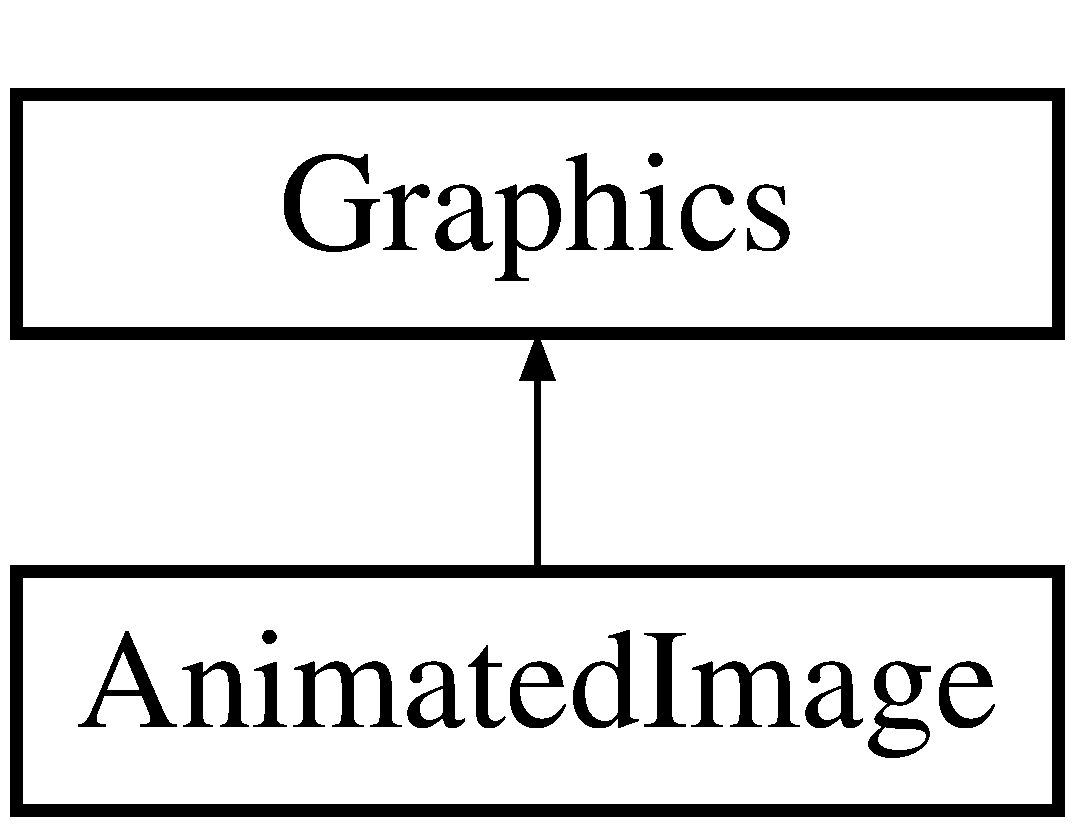
\includegraphics[height=2.000000cm]{class_animated_image}
\end{center}
\end{figure}
\subsection*{Public Member Functions}
\begin{DoxyCompactItemize}
\item 
\hyperlink{class_animated_image_a8b076dfb51777da777b77d2c5283ff6d}{Animated\+Image} (\hyperlink{class_screen}{Screen} \&\hyperlink{class_graphics_a7a73ddd0d3cf1b67fc54f303be017c3b}{w}, const uint8\+\_\+t $\ast$image, \hyperlink{classvector}{vector} \hyperlink{class_graphics_a88c2112c7a3db3ee56f4c7fe2cac6055}{location}=\hyperlink{classvector}{vector}(0, 0))
\begin{DoxyCompactList}\small\item\em \hyperlink{class_animated_image}{Animated\+Image} constructor\textquotesingle{}. \end{DoxyCompactList}\item 
void \hyperlink{class_animated_image_ab71f472b7a737d142fb6bf838dfc9818}{draw} ()
\begin{DoxyCompactList}\small\item\em draw the animated image on the screen. \end{DoxyCompactList}\item 
void \hyperlink{class_animated_image_a70cc2439dedf9e5fc366dd3a1534c167}{draw} (int update\+Interval, bool loop=false)
\begin{DoxyCompactList}\small\item\em draw the animated image on the screen. \end{DoxyCompactList}\item 
void \hyperlink{class_animated_image_a4f9a9236d7e2cec0b8b140743ac8340e}{draw\+Frame} (int)
\begin{DoxyCompactList}\small\item\em draw a specefiek frame on the screen. \end{DoxyCompactList}\item 
int \hyperlink{class_animated_image_af398536b19d4bdeefebfed02c77f47b3}{get\+Total\+Frames} ()
\begin{DoxyCompactList}\small\item\em Return number of frames of the animated\+Image. \end{DoxyCompactList}\end{DoxyCompactItemize}
\subsection*{Additional Inherited Members}


\subsection{Detailed Description}
Animate\+Image implementation for raw gif files. 

A class used to draw raw gif animations on the screen. 

\subsection{Constructor \& Destructor Documentation}
\index{Animated\+Image@{Animated\+Image}!Animated\+Image@{Animated\+Image}}
\index{Animated\+Image@{Animated\+Image}!Animated\+Image@{Animated\+Image}}
\subsubsection[{\texorpdfstring{Animated\+Image(\+Screen \&w, const uint8\+\_\+t $\ast$image, vector location=vector(0, 0))}{AnimatedImage(Screen &w, const uint8_t *image, vector location=vector(0, 0))}}]{\setlength{\rightskip}{0pt plus 5cm}Animated\+Image\+::\+Animated\+Image (
\begin{DoxyParamCaption}
\item[{{\bf Screen} \&}]{w, }
\item[{const uint8\+\_\+t $\ast$}]{image, }
\item[{{\bf vector}}]{location = {\ttfamily {\bf vector}(0,0)}}
\end{DoxyParamCaption}
)\hspace{0.3cm}{\ttfamily [inline]}}\hypertarget{class_animated_image_a8b076dfb51777da777b77d2c5283ff6d}{}\label{class_animated_image_a8b076dfb51777da777b77d2c5283ff6d}


\hyperlink{class_animated_image}{Animated\+Image} constructor\textquotesingle{}. 

\hyperlink{class_screen}{Screen} is the screen to draw on e.\+g. matrix. image is the raw gif file converted by a commandline script. After you included the conveted gif animation you can pass it to this function. Location is the location of animated image on the screen. 

\subsection{Member Function Documentation}
\index{Animated\+Image@{Animated\+Image}!draw@{draw}}
\index{draw@{draw}!Animated\+Image@{Animated\+Image}}
\subsubsection[{\texorpdfstring{draw()}{draw()}}]{\setlength{\rightskip}{0pt plus 5cm}void Animated\+Image\+::draw (
\begin{DoxyParamCaption}
{}
\end{DoxyParamCaption}
)\hspace{0.3cm}{\ttfamily [virtual]}}\hypertarget{class_animated_image_ab71f472b7a737d142fb6bf838dfc9818}{}\label{class_animated_image_ab71f472b7a737d142fb6bf838dfc9818}


draw the animated image on the screen. 

You do not need to swap buffers. Default loop is false and update interval is 10 milliseconds. 

Implements \hyperlink{class_graphics_a144fcecfe73dd5957c081dad42e1c11d}{Graphics}.

\index{Animated\+Image@{Animated\+Image}!draw@{draw}}
\index{draw@{draw}!Animated\+Image@{Animated\+Image}}
\subsubsection[{\texorpdfstring{draw(int update\+Interval, bool loop=false)}{draw(int updateInterval, bool loop=false)}}]{\setlength{\rightskip}{0pt plus 5cm}void Animated\+Image\+::draw (
\begin{DoxyParamCaption}
\item[{int}]{update\+Interval, }
\item[{bool}]{loop = {\ttfamily false}}
\end{DoxyParamCaption}
)}\hypertarget{class_animated_image_a70cc2439dedf9e5fc366dd3a1534c167}{}\label{class_animated_image_a70cc2439dedf9e5fc366dd3a1534c167}


draw the animated image on the screen. 

You do not need to swap buffers. update\+Interval is the delay between each frame. if loop is true the animation will be restarted when the last frame showed on the screen. \index{Animated\+Image@{Animated\+Image}!draw\+Frame@{draw\+Frame}}
\index{draw\+Frame@{draw\+Frame}!Animated\+Image@{Animated\+Image}}
\subsubsection[{\texorpdfstring{draw\+Frame(int)}{drawFrame(int)}}]{\setlength{\rightskip}{0pt plus 5cm}void Animated\+Image\+::draw\+Frame (
\begin{DoxyParamCaption}
\item[{int}]{frame}
\end{DoxyParamCaption}
)}\hypertarget{class_animated_image_a4f9a9236d7e2cec0b8b140743ac8340e}{}\label{class_animated_image_a4f9a9236d7e2cec0b8b140743ac8340e}


draw a specefiek frame on the screen. 

You need to swap buffer if double buffering is enabled. \index{Animated\+Image@{Animated\+Image}!get\+Total\+Frames@{get\+Total\+Frames}}
\index{get\+Total\+Frames@{get\+Total\+Frames}!Animated\+Image@{Animated\+Image}}
\subsubsection[{\texorpdfstring{get\+Total\+Frames()}{getTotalFrames()}}]{\setlength{\rightskip}{0pt plus 5cm}int Animated\+Image\+::get\+Total\+Frames (
\begin{DoxyParamCaption}
{}
\end{DoxyParamCaption}
)}\hypertarget{class_animated_image_af398536b19d4bdeefebfed02c77f47b3}{}\label{class_animated_image_af398536b19d4bdeefebfed02c77f47b3}


Return number of frames of the animated\+Image. 



The documentation for this class was generated from the following files\+:\begin{DoxyCompactItemize}
\item 
\hyperlink{_animated_image_8hpp}{Animated\+Image.\+hpp}\item 
\hyperlink{_animated_image_8cpp}{Animated\+Image.\+cpp}\end{DoxyCompactItemize}

\hypertarget{class_graphics}{}\section{Graphics Class Reference}
\label{class_graphics}\index{Graphics@{Graphics}}


The interface for other graphics objects.  




{\ttfamily \#include $<$Graphics.\+hpp$>$}

Inheritance diagram for Graphics\+:\begin{figure}[H]
\begin{center}
\leavevmode
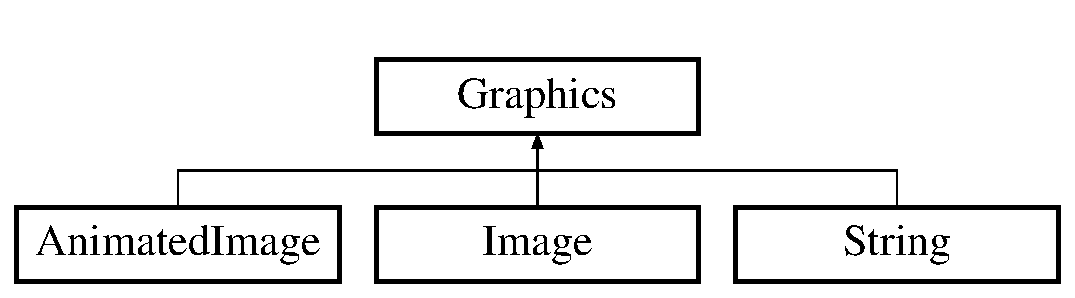
\includegraphics[height=2.000000cm]{class_graphics}
\end{center}
\end{figure}
\subsection*{Public Member Functions}
\begin{DoxyCompactItemize}
\item 
\hyperlink{class_graphics_a1947a936c3beadc6d2cdf156243e25ee}{Graphics} (\hyperlink{class_screen}{Screen} \&\hyperlink{class_graphics_a7a73ddd0d3cf1b67fc54f303be017c3b}{w}, \hyperlink{classvector}{vector} \hyperlink{class_graphics_a9a857a75730ffd8d473ca7624425d92a}{size}, \hyperlink{classvector}{vector} \hyperlink{class_graphics_a88c2112c7a3db3ee56f4c7fe2cac6055}{location})
\begin{DoxyCompactList}\small\item\em \hyperlink{class_graphics}{Graphics} constructor. \end{DoxyCompactList}\item 
virtual void \hyperlink{class_graphics_a144fcecfe73dd5957c081dad42e1c11d}{draw} ()=0
\begin{DoxyCompactList}\small\item\em draw graphics object on the screen. \end{DoxyCompactList}\item 
\hyperlink{classvector}{vector} \hyperlink{class_graphics_aad09e009edd57dbe96858b261e9b3605}{get\+Size} () const 
\begin{DoxyCompactList}\small\item\em return the size of a graphics object. \end{DoxyCompactList}\item 
\hyperlink{classvector}{vector} \hyperlink{class_graphics_a80b0b5536416cf79b0c9da98e419cacd}{get\+Location} () const 
\begin{DoxyCompactList}\small\item\em return the location of a graphics object. \end{DoxyCompactList}\item 
\hyperlink{class_screen}{Screen} \& \hyperlink{class_graphics_a0cfd8e41ff0a1c92ebd30089d7dd6bab}{get\+Screen} () const 
\begin{DoxyCompactList}\small\item\em return the screen used by graphics object \end{DoxyCompactList}\item 
void \hyperlink{class_graphics_a6b89d760e95a1aad37ac1996c3f9d7ea}{set\+Location} (\hyperlink{classvector}{vector} l)
\begin{DoxyCompactList}\small\item\em change the location of a graphics object. \end{DoxyCompactList}\item 
void \hyperlink{class_graphics_a473b0893180b72e3e506ff9e09618797}{set\+Size} (\hyperlink{classvector}{vector} s)
\begin{DoxyCompactList}\small\item\em change the size of a graphics object \end{DoxyCompactList}\end{DoxyCompactItemize}
\subsection*{Protected Attributes}
\begin{DoxyCompactItemize}
\item 
\hyperlink{class_screen}{Screen} \& \hyperlink{class_graphics_a7a73ddd0d3cf1b67fc54f303be017c3b}{w}
\item 
\hyperlink{classvector}{vector} \hyperlink{class_graphics_a9a857a75730ffd8d473ca7624425d92a}{size}
\item 
\hyperlink{classvector}{vector} \hyperlink{class_graphics_a88c2112c7a3db3ee56f4c7fe2cac6055}{location}
\end{DoxyCompactItemize}


\subsection{Detailed Description}
The interface for other graphics objects. 

\hyperlink{class_graphics}{Graphics} class is an abstract class used as an interface for other graphic objects like \hyperlink{class_image}{Image}, \hyperlink{class_string}{String} and Animated \hyperlink{class_image}{Image}. This is an abstract class. It can be used only as a base for other objects. 

\subsection{Constructor \& Destructor Documentation}
\index{Graphics@{Graphics}!Graphics@{Graphics}}
\index{Graphics@{Graphics}!Graphics@{Graphics}}
\subsubsection[{\texorpdfstring{Graphics(\+Screen \&w, vector size, vector location)}{Graphics(Screen &w, vector size, vector location)}}]{\setlength{\rightskip}{0pt plus 5cm}Graphics\+::\+Graphics (
\begin{DoxyParamCaption}
\item[{{\bf Screen} \&}]{w, }
\item[{{\bf vector}}]{size, }
\item[{{\bf vector}}]{location}
\end{DoxyParamCaption}
)\hspace{0.3cm}{\ttfamily [inline]}}\hypertarget{class_graphics_a1947a936c3beadc6d2cdf156243e25ee}{}\label{class_graphics_a1947a936c3beadc6d2cdf156243e25ee}


\hyperlink{class_graphics}{Graphics} constructor. 

\hyperlink{class_screen}{Screen} to draw graphics on it e.\+g. matrix. Size is the size of object and location is the pixels position on the screen. 

\subsection{Member Function Documentation}
\index{Graphics@{Graphics}!draw@{draw}}
\index{draw@{draw}!Graphics@{Graphics}}
\subsubsection[{\texorpdfstring{draw()=0}{draw()=0}}]{\setlength{\rightskip}{0pt plus 5cm}virtual void Graphics\+::draw (
\begin{DoxyParamCaption}
{}
\end{DoxyParamCaption}
)\hspace{0.3cm}{\ttfamily [pure virtual]}}\hypertarget{class_graphics_a144fcecfe73dd5957c081dad42e1c11d}{}\label{class_graphics_a144fcecfe73dd5957c081dad42e1c11d}


draw graphics object on the screen. 



Implemented in \hyperlink{class_string_a6f00d1cdc1842feb404809c717a62581}{String}, \hyperlink{class_animated_image_ab71f472b7a737d142fb6bf838dfc9818}{Animated\+Image}, and \hyperlink{class_image_af67dbed0b509945e278bdd88088615cf}{Image}.

\index{Graphics@{Graphics}!get\+Location@{get\+Location}}
\index{get\+Location@{get\+Location}!Graphics@{Graphics}}
\subsubsection[{\texorpdfstring{get\+Location() const }{getLocation() const }}]{\setlength{\rightskip}{0pt plus 5cm}{\bf vector} Graphics\+::get\+Location (
\begin{DoxyParamCaption}
{}
\end{DoxyParamCaption}
) const\hspace{0.3cm}{\ttfamily [inline]}}\hypertarget{class_graphics_a80b0b5536416cf79b0c9da98e419cacd}{}\label{class_graphics_a80b0b5536416cf79b0c9da98e419cacd}


return the location of a graphics object. 

\index{Graphics@{Graphics}!get\+Screen@{get\+Screen}}
\index{get\+Screen@{get\+Screen}!Graphics@{Graphics}}
\subsubsection[{\texorpdfstring{get\+Screen() const }{getScreen() const }}]{\setlength{\rightskip}{0pt plus 5cm}{\bf Screen}\& Graphics\+::get\+Screen (
\begin{DoxyParamCaption}
{}
\end{DoxyParamCaption}
) const\hspace{0.3cm}{\ttfamily [inline]}}\hypertarget{class_graphics_a0cfd8e41ff0a1c92ebd30089d7dd6bab}{}\label{class_graphics_a0cfd8e41ff0a1c92ebd30089d7dd6bab}


return the screen used by graphics object 

\index{Graphics@{Graphics}!get\+Size@{get\+Size}}
\index{get\+Size@{get\+Size}!Graphics@{Graphics}}
\subsubsection[{\texorpdfstring{get\+Size() const }{getSize() const }}]{\setlength{\rightskip}{0pt plus 5cm}{\bf vector} Graphics\+::get\+Size (
\begin{DoxyParamCaption}
{}
\end{DoxyParamCaption}
) const\hspace{0.3cm}{\ttfamily [inline]}}\hypertarget{class_graphics_aad09e009edd57dbe96858b261e9b3605}{}\label{class_graphics_aad09e009edd57dbe96858b261e9b3605}


return the size of a graphics object. 

\index{Graphics@{Graphics}!set\+Location@{set\+Location}}
\index{set\+Location@{set\+Location}!Graphics@{Graphics}}
\subsubsection[{\texorpdfstring{set\+Location(vector l)}{setLocation(vector l)}}]{\setlength{\rightskip}{0pt plus 5cm}void Graphics\+::set\+Location (
\begin{DoxyParamCaption}
\item[{{\bf vector}}]{l}
\end{DoxyParamCaption}
)\hspace{0.3cm}{\ttfamily [inline]}}\hypertarget{class_graphics_a6b89d760e95a1aad37ac1996c3f9d7ea}{}\label{class_graphics_a6b89d760e95a1aad37ac1996c3f9d7ea}


change the location of a graphics object. 

\index{Graphics@{Graphics}!set\+Size@{set\+Size}}
\index{set\+Size@{set\+Size}!Graphics@{Graphics}}
\subsubsection[{\texorpdfstring{set\+Size(vector s)}{setSize(vector s)}}]{\setlength{\rightskip}{0pt plus 5cm}void Graphics\+::set\+Size (
\begin{DoxyParamCaption}
\item[{{\bf vector}}]{s}
\end{DoxyParamCaption}
)\hspace{0.3cm}{\ttfamily [inline]}}\hypertarget{class_graphics_a473b0893180b72e3e506ff9e09618797}{}\label{class_graphics_a473b0893180b72e3e506ff9e09618797}


change the size of a graphics object 



\subsection{Member Data Documentation}
\index{Graphics@{Graphics}!location@{location}}
\index{location@{location}!Graphics@{Graphics}}
\subsubsection[{\texorpdfstring{location}{location}}]{\setlength{\rightskip}{0pt plus 5cm}{\bf vector} Graphics\+::location\hspace{0.3cm}{\ttfamily [protected]}}\hypertarget{class_graphics_a88c2112c7a3db3ee56f4c7fe2cac6055}{}\label{class_graphics_a88c2112c7a3db3ee56f4c7fe2cac6055}
\index{Graphics@{Graphics}!size@{size}}
\index{size@{size}!Graphics@{Graphics}}
\subsubsection[{\texorpdfstring{size}{size}}]{\setlength{\rightskip}{0pt plus 5cm}{\bf vector} Graphics\+::size\hspace{0.3cm}{\ttfamily [protected]}}\hypertarget{class_graphics_a9a857a75730ffd8d473ca7624425d92a}{}\label{class_graphics_a9a857a75730ffd8d473ca7624425d92a}
\index{Graphics@{Graphics}!w@{w}}
\index{w@{w}!Graphics@{Graphics}}
\subsubsection[{\texorpdfstring{w}{w}}]{\setlength{\rightskip}{0pt plus 5cm}{\bf Screen}\& Graphics\+::w\hspace{0.3cm}{\ttfamily [protected]}}\hypertarget{class_graphics_a7a73ddd0d3cf1b67fc54f303be017c3b}{}\label{class_graphics_a7a73ddd0d3cf1b67fc54f303be017c3b}


The documentation for this class was generated from the following file\+:\begin{DoxyCompactItemize}
\item 
\hyperlink{_graphics_8hpp}{Graphics.\+hpp}\end{DoxyCompactItemize}

\hypertarget{class_image}{}\section{Image Class Reference}
\label{class_image}\index{Image@{Image}}


Implementation for raw image files.  




{\ttfamily \#include $<$Image.\+hpp$>$}

Inheritance diagram for Image\+:\begin{figure}[H]
\begin{center}
\leavevmode
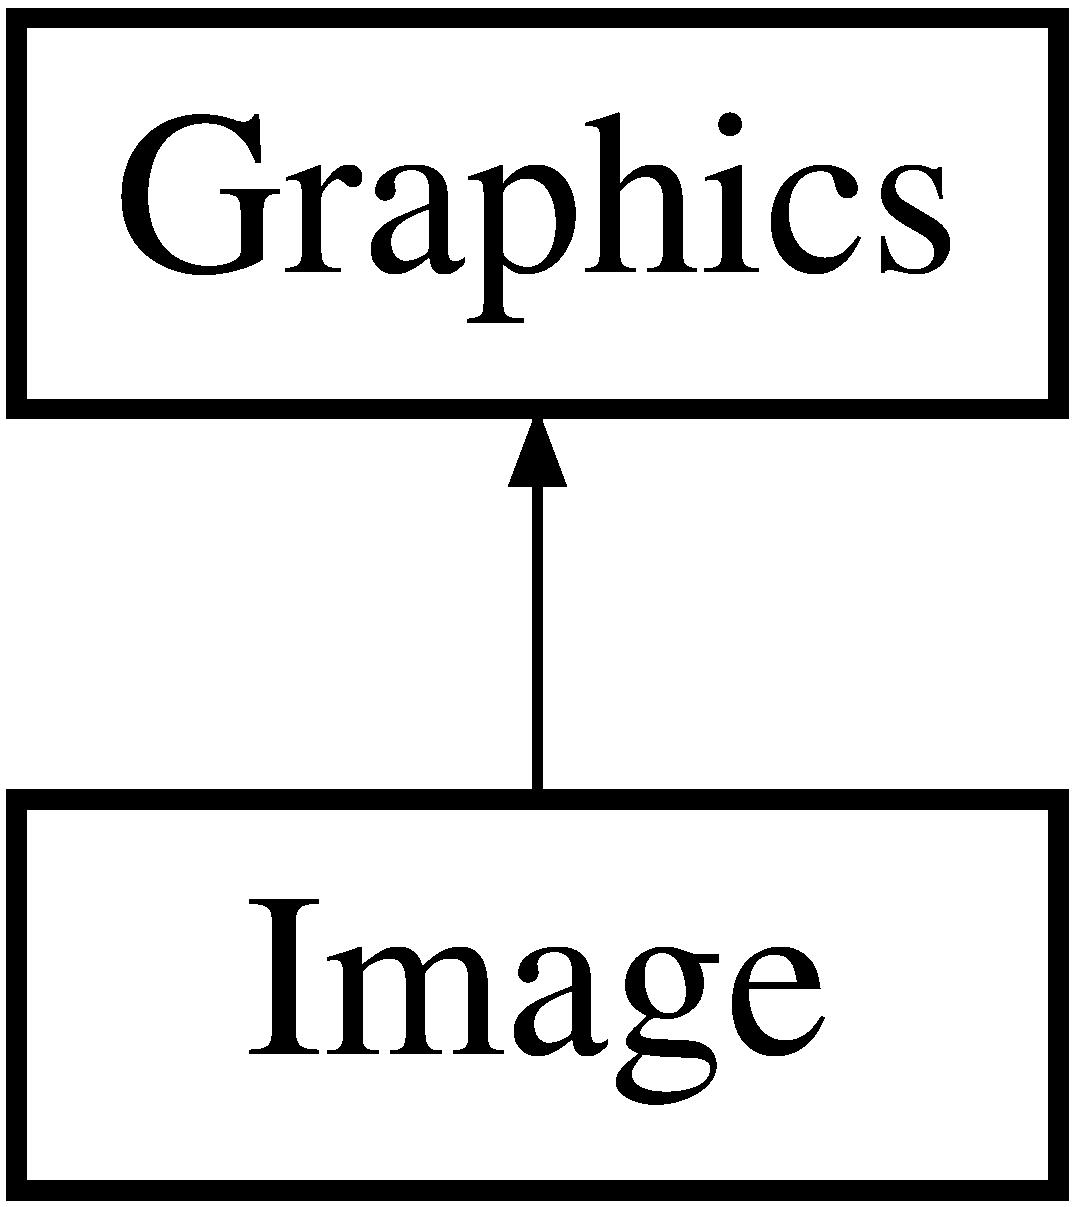
\includegraphics[height=2.000000cm]{class_image}
\end{center}
\end{figure}
\subsection*{Public Member Functions}
\begin{DoxyCompactItemize}
\item 
\hyperlink{class_image_aaa4504304ed8b2fa33bb6b4fc52a2199}{Image} (\hyperlink{class_screen}{Screen} \&\hyperlink{class_graphics_a7a73ddd0d3cf1b67fc54f303be017c3b}{w}, const uint8\+\_\+t $\ast$im, \hyperlink{classvector}{vector} \hyperlink{class_graphics_a88c2112c7a3db3ee56f4c7fe2cac6055}{location}=\hyperlink{classvector}{vector}(0, 0))
\begin{DoxyCompactList}\small\item\em \hyperlink{class_image}{Image} constructors. \end{DoxyCompactList}\item 
void \hyperlink{class_image_af67dbed0b509945e278bdd88088615cf}{draw} () override
\begin{DoxyCompactList}\small\item\em print the image on the screen. \end{DoxyCompactList}\end{DoxyCompactItemize}
\subsection*{Additional Inherited Members}


\subsection{Detailed Description}
Implementation for raw image files. 

This class is used to draw photos on the screen. 

\subsection{Constructor \& Destructor Documentation}
\index{Image@{Image}!Image@{Image}}
\index{Image@{Image}!Image@{Image}}
\subsubsection[{\texorpdfstring{Image(\+Screen \&w, const uint8\+\_\+t $\ast$im, vector location=vector(0, 0))}{Image(Screen &w, const uint8_t *im, vector location=vector(0, 0))}}]{\setlength{\rightskip}{0pt plus 5cm}Image\+::\+Image (
\begin{DoxyParamCaption}
\item[{{\bf Screen} \&}]{w, }
\item[{const uint8\+\_\+t $\ast$}]{im, }
\item[{{\bf vector}}]{location = {\ttfamily {\bf vector}(0,0)}}
\end{DoxyParamCaption}
)\hspace{0.3cm}{\ttfamily [inline]}}\hypertarget{class_image_aaa4504304ed8b2fa33bb6b4fc52a2199}{}\label{class_image_aaa4504304ed8b2fa33bb6b4fc52a2199}


\hyperlink{class_image}{Image} constructors. 

\hyperlink{class_screen}{Screen} to draw image on it, e.\+g. matrix. image is a raw photo converted by a command line script. You have to include a raw file and then pass it to this function. Location is the location to draw image on the screen. 

\subsection{Member Function Documentation}
\index{Image@{Image}!draw@{draw}}
\index{draw@{draw}!Image@{Image}}
\subsubsection[{\texorpdfstring{draw() override}{draw() override}}]{\setlength{\rightskip}{0pt plus 5cm}void Image\+::draw (
\begin{DoxyParamCaption}
{}
\end{DoxyParamCaption}
)\hspace{0.3cm}{\ttfamily [override]}, {\ttfamily [virtual]}}\hypertarget{class_image_af67dbed0b509945e278bdd88088615cf}{}\label{class_image_af67dbed0b509945e278bdd88088615cf}


print the image on the screen. 

If you enabled a double buffering you have to swap buffers to draw the image on the screen. 

Implements \hyperlink{class_graphics_a144fcecfe73dd5957c081dad42e1c11d}{Graphics}.



The documentation for this class was generated from the following files\+:\begin{DoxyCompactItemize}
\item 
\hyperlink{_image_8hpp}{Image.\+hpp}\item 
\hyperlink{_image_8cpp}{Image.\+cpp}\end{DoxyCompactItemize}

\hypertarget{classmatrix}{}\section{matrix Class Reference}
\label{classmatrix}\index{matrix@{matrix}}


Led matrix implementation for the abstract class \hyperlink{class_screen}{Screen}.  




{\ttfamily \#include $<$matrix.\+hpp$>$}

Inheritance diagram for matrix\+:\begin{figure}[H]
\begin{center}
\leavevmode
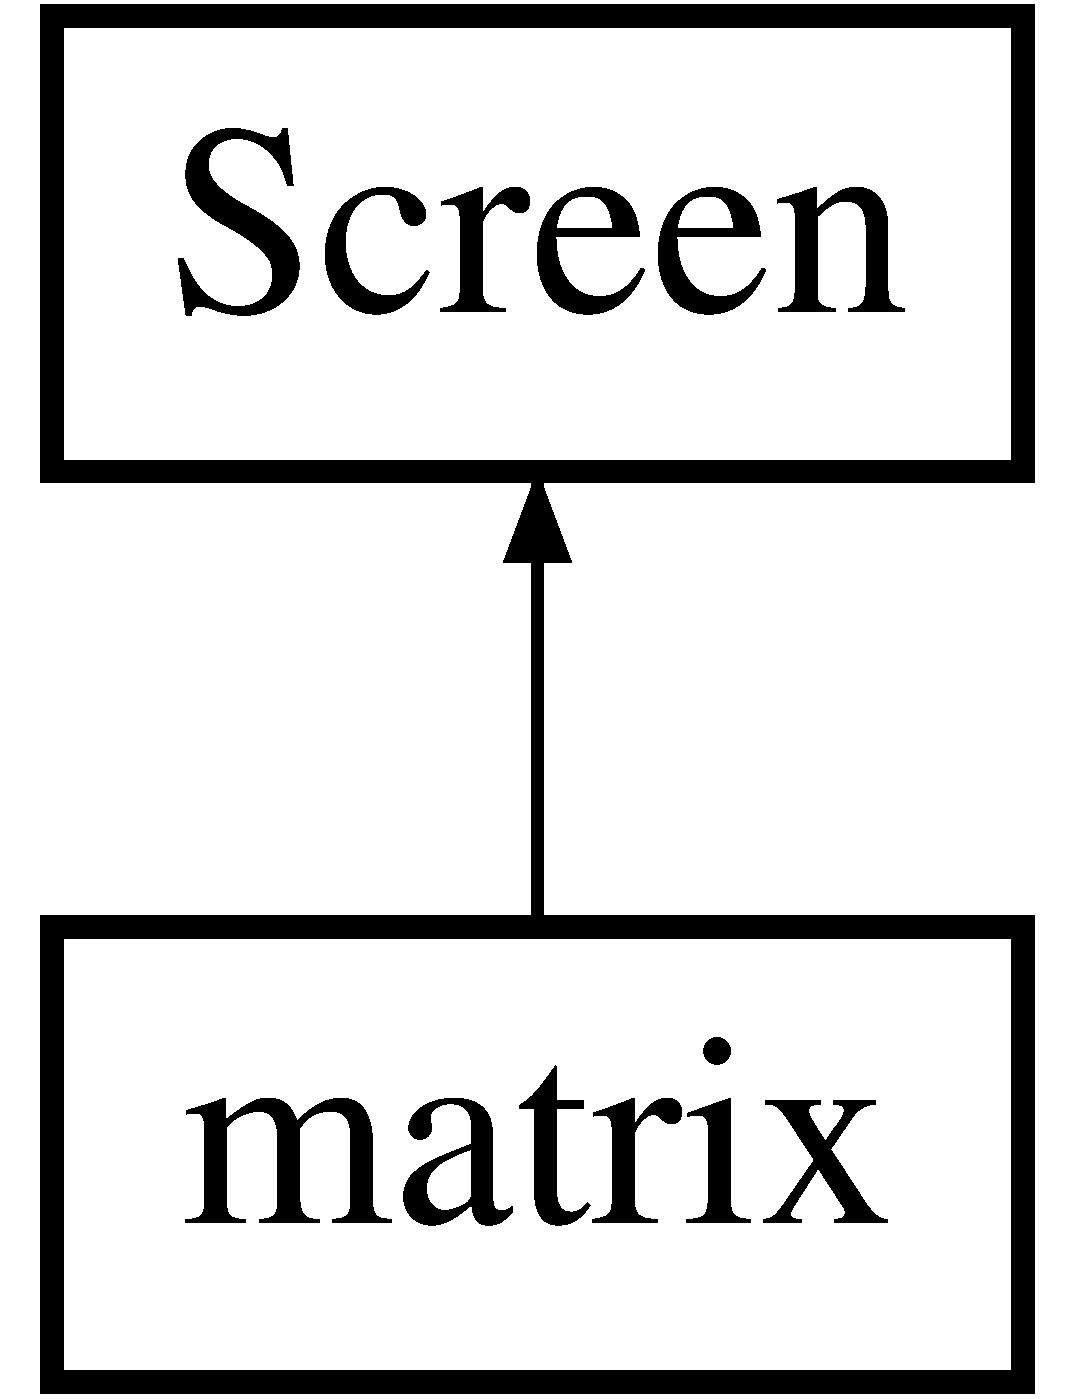
\includegraphics[height=2.000000cm]{classmatrix}
\end{center}
\end{figure}
\subsection*{Public Member Functions}
\begin{DoxyCompactItemize}
\item 
\hyperlink{classmatrix_a4e54abccfd55d40a3caebb47b1bf96a0}{matrix} (int \hyperlink{class_screen_a49be8f8ccf7ed7a3151a761495c0ce21}{width}, int \hyperlink{class_screen_a55405920693276db8fbdbf3a903b8d2f}{height}, bool double\+\_\+buffer)
\begin{DoxyCompactList}\small\item\em Matrix constructor with default wiring. \end{DoxyCompactList}\item 
\hyperlink{classmatrix_a29a4203237fd9480a42b435fb504b2b5}{matrix} (int \hyperlink{class_screen_a49be8f8ccf7ed7a3151a761495c0ce21}{width}, int \hyperlink{class_screen_a55405920693276db8fbdbf3a903b8d2f}{height}, bool double\+\_\+buffer, target\+::pin\+\_\+out \+\_\+lat, target\+::pin\+\_\+out \+\_\+oe, target\+::pin\+\_\+out \+\_\+clk, target\+::pin\+\_\+out \+\_\+selA, target\+::pin\+\_\+out \+\_\+selB, target\+::pin\+\_\+out \+\_\+selC, target\+::pin\+\_\+out \+\_\+selD, target\+::pin\+\_\+out \+\_\+b1, target\+::pin\+\_\+out \+\_\+g1, target\+::pin\+\_\+out \+\_\+r1, target\+::pin\+\_\+out \+\_\+b2, target\+::pin\+\_\+out \+\_\+g2, target\+::pin\+\_\+out \+\_\+r2)
\begin{DoxyCompactList}\small\item\em Matrix constructor with custom wiring. \end{DoxyCompactList}\item 
void \hyperlink{classmatrix_a9e12daa9f177f70cecfeae60770eb59a}{draw\+Pixel} (int x, int y, uint8\+\_\+t rc, uint8\+\_\+t gc, uint8\+\_\+t bc) override
\begin{DoxyCompactList}\small\item\em Draw a given pixel with a color R G B. \end{DoxyCompactList}\item 
void \hyperlink{classmatrix_a505fdd2958c4be8cf2ceaf19873358f9}{draw\+Pixel} (int x, int y, uint32\+\_\+t color)
\begin{DoxyCompactList}\small\item\em Draw a pixel with a hexadecimale color. \end{DoxyCompactList}\item 
void \hyperlink{classmatrix_afbb1e0fe6c1ad426879c5019b39f896e}{fill\+Screen} (uint8\+\_\+t r, uint8\+\_\+t g, uint8\+\_\+t b) override
\begin{DoxyCompactList}\small\item\em Fill the entire screen with r g b colors. \end{DoxyCompactList}\item 
void \hyperlink{classmatrix_a1a44a0f6011c61daa50391cda8d662d9}{fill\+Screen} (uint32\+\_\+t color)
\begin{DoxyCompactList}\small\item\em Fill the entire screen with a hexa or decimal color. \end{DoxyCompactList}\item 
void \hyperlink{classmatrix_af7e01d4f030990aba4e57af5085bd25c}{clear} () override
\begin{DoxyCompactList}\small\item\em Clear the entire screen. \end{DoxyCompactList}\item 
void \hyperlink{classmatrix_a191f64280f94a2fba62ad92edf6d038a}{start} () override
\begin{DoxyCompactList}\small\item\em Start the auto update of the screen. \end{DoxyCompactList}\item 
void \hyperlink{classmatrix_a3e791088f813e071a60dca840b6b3767}{stop} () override
\begin{DoxyCompactList}\small\item\em Stop the auto update of the screen. \end{DoxyCompactList}\item 
void \hyperlink{classmatrix_a371a4877409c2710021cfa3c226e63fb}{swap\+\_\+buffer} (bool copy) override
\begin{DoxyCompactList}\small\item\em Swap the front buffer with the back buffer. \end{DoxyCompactList}\item 
void \hyperlink{classmatrix_a55827c936f54e69487cc52b83a2311c3}{update} () override
\begin{DoxyCompactList}\small\item\em Update the screen. \end{DoxyCompactList}\item 
void \hyperlink{classmatrix_a32dade57d6aea1b4bb9aba2e5b4992ca}{update2} ()
\item 
bool \hyperlink{classmatrix_a94d0258f761e50a832b84bc12704c7eb}{is\+\_\+using\+\_\+default\+\_\+pins} ()
\end{DoxyCompactItemize}
\subsection*{Additional Inherited Members}


\subsection{Detailed Description}
Led matrix implementation for the abstract class \hyperlink{class_screen}{Screen}. 

This class contains an implementation for the led matrix 32x64 but also for other led matrixes like 32x32 and 16x32. 

\subsection{Constructor \& Destructor Documentation}
\index{matrix@{matrix}!matrix@{matrix}}
\index{matrix@{matrix}!matrix@{matrix}}
\subsubsection[{\texorpdfstring{matrix(int width, int height, bool double\+\_\+buffer)}{matrix(int width, int height, bool double_buffer)}}]{\setlength{\rightskip}{0pt plus 5cm}matrix\+::matrix (
\begin{DoxyParamCaption}
\item[{int}]{width, }
\item[{int}]{height, }
\item[{bool}]{double\+\_\+buffer}
\end{DoxyParamCaption}
)}\hypertarget{classmatrix_a4e54abccfd55d40a3caebb47b1bf96a0}{}\label{classmatrix_a4e54abccfd55d40a3caebb47b1bf96a0}


Matrix constructor with default wiring. 

matrix constructor with given width, height and the posibility to choose a double buffer. if you chose to use a double buffer you always write into the back buffer. So you can\textquotesingle{}t see the result unless you swap the buffers with swap\+\_\+buffer methode. \index{matrix@{matrix}!matrix@{matrix}}
\index{matrix@{matrix}!matrix@{matrix}}
\subsubsection[{\texorpdfstring{matrix(int width, int height, bool double\+\_\+buffer, target\+::pin\+\_\+out \+\_\+lat, target\+::pin\+\_\+out \+\_\+oe, target\+::pin\+\_\+out \+\_\+clk, target\+::pin\+\_\+out \+\_\+sel\+A, target\+::pin\+\_\+out \+\_\+sel\+B, target\+::pin\+\_\+out \+\_\+sel\+C, target\+::pin\+\_\+out \+\_\+sel\+D, target\+::pin\+\_\+out \+\_\+b1, target\+::pin\+\_\+out \+\_\+g1, target\+::pin\+\_\+out \+\_\+r1, target\+::pin\+\_\+out \+\_\+b2, target\+::pin\+\_\+out \+\_\+g2, target\+::pin\+\_\+out \+\_\+r2)}{matrix(int width, int height, bool double_buffer, target::pin_out _lat, target::pin_out _oe, target::pin_out _clk, target::pin_out _selA, target::pin_out _selB, target::pin_out _selC, target::pin_out _selD, target::pin_out _b1, target::pin_out _g1, target::pin_out _r1, target::pin_out _b2, target::pin_out _g2, target::pin_out _r2)}}]{\setlength{\rightskip}{0pt plus 5cm}matrix\+::matrix (
\begin{DoxyParamCaption}
\item[{int}]{width, }
\item[{int}]{height, }
\item[{bool}]{double\+\_\+buffer, }
\item[{target\+::pin\+\_\+out}]{\+\_\+lat, }
\item[{target\+::pin\+\_\+out}]{\+\_\+oe, }
\item[{target\+::pin\+\_\+out}]{\+\_\+clk, }
\item[{target\+::pin\+\_\+out}]{\+\_\+selA, }
\item[{target\+::pin\+\_\+out}]{\+\_\+selB, }
\item[{target\+::pin\+\_\+out}]{\+\_\+selC, }
\item[{target\+::pin\+\_\+out}]{\+\_\+selD, }
\item[{target\+::pin\+\_\+out}]{\+\_\+b1, }
\item[{target\+::pin\+\_\+out}]{\+\_\+g1, }
\item[{target\+::pin\+\_\+out}]{\+\_\+r1, }
\item[{target\+::pin\+\_\+out}]{\+\_\+b2, }
\item[{target\+::pin\+\_\+out}]{\+\_\+g2, }
\item[{target\+::pin\+\_\+out}]{\+\_\+r2}
\end{DoxyParamCaption}
)}\hypertarget{classmatrix_a29a4203237fd9480a42b435fb504b2b5}{}\label{classmatrix_a29a4203237fd9480a42b435fb504b2b5}


Matrix constructor with custom wiring. 

matrix constructor with given width, height and the posibility to choose a double buffer. if you chose to use a double buffer you always write into the back buffer. So you can\textquotesingle{}t see the result unless you swap the buffers with swap\+\_\+buffer methode. 

\subsection{Member Function Documentation}
\index{matrix@{matrix}!clear@{clear}}
\index{clear@{clear}!matrix@{matrix}}
\subsubsection[{\texorpdfstring{clear() override}{clear() override}}]{\setlength{\rightskip}{0pt plus 5cm}void matrix\+::clear (
\begin{DoxyParamCaption}
{}
\end{DoxyParamCaption}
)\hspace{0.3cm}{\ttfamily [override]}, {\ttfamily [virtual]}}\hypertarget{classmatrix_af7e01d4f030990aba4e57af5085bd25c}{}\label{classmatrix_af7e01d4f030990aba4e57af5085bd25c}


Clear the entire screen. 

This function clears the back buffer if double buffer is enabled otherwise clears the front buffer. 

Implements \hyperlink{class_screen_aeeb33479781ffe35c4f1c90cd66824aa}{Screen}.

\index{matrix@{matrix}!draw\+Pixel@{draw\+Pixel}}
\index{draw\+Pixel@{draw\+Pixel}!matrix@{matrix}}
\subsubsection[{\texorpdfstring{draw\+Pixel(int x, int y, uint8\+\_\+t rc, uint8\+\_\+t gc, uint8\+\_\+t bc) override}{drawPixel(int x, int y, uint8_t rc, uint8_t gc, uint8_t bc) override}}]{\setlength{\rightskip}{0pt plus 5cm}void matrix\+::draw\+Pixel (
\begin{DoxyParamCaption}
\item[{int}]{x, }
\item[{int}]{y, }
\item[{uint8\+\_\+t}]{rc, }
\item[{uint8\+\_\+t}]{gc, }
\item[{uint8\+\_\+t}]{bc}
\end{DoxyParamCaption}
)\hspace{0.3cm}{\ttfamily [override]}, {\ttfamily [virtual]}}\hypertarget{classmatrix_a9e12daa9f177f70cecfeae60770eb59a}{}\label{classmatrix_a9e12daa9f177f70cecfeae60770eb59a}


Draw a given pixel with a color R G B. 

the first int argument is the width position and the second int argument is the height position of a pixel. rgb colors are between 0 and 255. This function writes always into the back buffer if double buffer is enabled, otherwise writes into the front buffer. 

Implements \hyperlink{class_screen_a29b3d5ac1b1f9965daa31be3acb2058e}{Screen}.

\index{matrix@{matrix}!draw\+Pixel@{draw\+Pixel}}
\index{draw\+Pixel@{draw\+Pixel}!matrix@{matrix}}
\subsubsection[{\texorpdfstring{draw\+Pixel(int x, int y, uint32\+\_\+t color)}{drawPixel(int x, int y, uint32_t color)}}]{\setlength{\rightskip}{0pt plus 5cm}void matrix\+::draw\+Pixel (
\begin{DoxyParamCaption}
\item[{int}]{x, }
\item[{int}]{y, }
\item[{uint32\+\_\+t}]{color}
\end{DoxyParamCaption}
)\hspace{0.3cm}{\ttfamily [virtual]}}\hypertarget{classmatrix_a505fdd2958c4be8cf2ceaf19873358f9}{}\label{classmatrix_a505fdd2958c4be8cf2ceaf19873358f9}


Draw a pixel with a hexadecimale color. 

the first int argument is the width position and the second is the height position of a pixel. color is rgb is hexa or decimale. This function writes always into the back buffer if double buffer is enabled, otherwise writes into the front buffer. 

Implements \hyperlink{class_screen_a01e3bb789c4169dec25e842179b7b115}{Screen}.

\index{matrix@{matrix}!fill\+Screen@{fill\+Screen}}
\index{fill\+Screen@{fill\+Screen}!matrix@{matrix}}
\subsubsection[{\texorpdfstring{fill\+Screen(uint8\+\_\+t r, uint8\+\_\+t g, uint8\+\_\+t b) override}{fillScreen(uint8_t r, uint8_t g, uint8_t b) override}}]{\setlength{\rightskip}{0pt plus 5cm}void matrix\+::fill\+Screen (
\begin{DoxyParamCaption}
\item[{uint8\+\_\+t}]{r, }
\item[{uint8\+\_\+t}]{g, }
\item[{uint8\+\_\+t}]{b}
\end{DoxyParamCaption}
)\hspace{0.3cm}{\ttfamily [override]}, {\ttfamily [virtual]}}\hypertarget{classmatrix_afbb1e0fe6c1ad426879c5019b39f896e}{}\label{classmatrix_afbb1e0fe6c1ad426879c5019b39f896e}


Fill the entire screen with r g b colors. 

This function fills the back buffer if double buffer is enabled otherwise clears the front buffer. 

Reimplemented from \hyperlink{class_screen_a7561ce620e5dd79717bced178e32e139}{Screen}.

\index{matrix@{matrix}!fill\+Screen@{fill\+Screen}}
\index{fill\+Screen@{fill\+Screen}!matrix@{matrix}}
\subsubsection[{\texorpdfstring{fill\+Screen(uint32\+\_\+t color)}{fillScreen(uint32_t color)}}]{\setlength{\rightskip}{0pt plus 5cm}void matrix\+::fill\+Screen (
\begin{DoxyParamCaption}
\item[{uint32\+\_\+t}]{color}
\end{DoxyParamCaption}
)\hspace{0.3cm}{\ttfamily [virtual]}}\hypertarget{classmatrix_a1a44a0f6011c61daa50391cda8d662d9}{}\label{classmatrix_a1a44a0f6011c61daa50391cda8d662d9}


Fill the entire screen with a hexa or decimal color. 

This function fills the back buffer if double buffer is enabled otherwise clears the front buffer. 

Reimplemented from \hyperlink{class_screen_a6e3a21e03ec2a378c9be90b7a0a149b2}{Screen}.

\index{matrix@{matrix}!is\+\_\+using\+\_\+default\+\_\+pins@{is\+\_\+using\+\_\+default\+\_\+pins}}
\index{is\+\_\+using\+\_\+default\+\_\+pins@{is\+\_\+using\+\_\+default\+\_\+pins}!matrix@{matrix}}
\subsubsection[{\texorpdfstring{is\+\_\+using\+\_\+default\+\_\+pins()}{is_using_default_pins()}}]{\setlength{\rightskip}{0pt plus 5cm}bool matrix\+::is\+\_\+using\+\_\+default\+\_\+pins (
\begin{DoxyParamCaption}
{}
\end{DoxyParamCaption}
)\hspace{0.3cm}{\ttfamily [inline]}}\hypertarget{classmatrix_a94d0258f761e50a832b84bc12704c7eb}{}\label{classmatrix_a94d0258f761e50a832b84bc12704c7eb}
\index{matrix@{matrix}!start@{start}}
\index{start@{start}!matrix@{matrix}}
\subsubsection[{\texorpdfstring{start() override}{start() override}}]{\setlength{\rightskip}{0pt plus 5cm}void matrix\+::start (
\begin{DoxyParamCaption}
{}
\end{DoxyParamCaption}
)\hspace{0.3cm}{\ttfamily [override]}, {\ttfamily [virtual]}}\hypertarget{classmatrix_a191f64280f94a2fba62ad92edf6d038a}{}\label{classmatrix_a191f64280f94a2fba62ad92edf6d038a}


Start the auto update of the screen. 

The led matrix needs to be updated constantly. This function does the job of updating the screen with a frequenty of 200 HZ. 

Reimplemented from \hyperlink{class_screen_a72c3f62745b4b863edb9e95d10057429}{Screen}.

\index{matrix@{matrix}!stop@{stop}}
\index{stop@{stop}!matrix@{matrix}}
\subsubsection[{\texorpdfstring{stop() override}{stop() override}}]{\setlength{\rightskip}{0pt plus 5cm}void matrix\+::stop (
\begin{DoxyParamCaption}
{}
\end{DoxyParamCaption}
)\hspace{0.3cm}{\ttfamily [override]}, {\ttfamily [virtual]}}\hypertarget{classmatrix_a3e791088f813e071a60dca840b6b3767}{}\label{classmatrix_a3e791088f813e071a60dca840b6b3767}


Stop the auto update of the screen. 

If you stop the auto update of the screen the current picture on the screen will be removed and maybe only one row or twoo rows of the led matrix remains light. 

Reimplemented from \hyperlink{class_screen_a38efb55f9bcb9d7181edb580ad7a77fc}{Screen}.

\index{matrix@{matrix}!swap\+\_\+buffer@{swap\+\_\+buffer}}
\index{swap\+\_\+buffer@{swap\+\_\+buffer}!matrix@{matrix}}
\subsubsection[{\texorpdfstring{swap\+\_\+buffer(bool copy) override}{swap_buffer(bool copy) override}}]{\setlength{\rightskip}{0pt plus 5cm}void matrix\+::swap\+\_\+buffer (
\begin{DoxyParamCaption}
\item[{bool}]{copy}
\end{DoxyParamCaption}
)\hspace{0.3cm}{\ttfamily [override]}, {\ttfamily [virtual]}}\hypertarget{classmatrix_a371a4877409c2710021cfa3c226e63fb}{}\label{classmatrix_a371a4877409c2710021cfa3c226e63fb}


Swap the front buffer with the back buffer. 

If double buffer is enabled, you can swap the front buffer and the back buffer with this function. If you need to copy the values of the updated buffer into the new back buffer you need to pass true to the copy varianle. But if you only need to swap the front buffer with the back buffer and you don\textquotesingle{}t care about the old buffer (maybe because you clear the screen afterwards) the pass false to the copy variable. To avoid \char`\"{}tearing\char`\"{} swapping of buffers takes place at the end of a complete screen refresh cycle. N\+O\+TE\+: This function doesn\textquotesingle{}t have any effect if you didn\textquotesingle{}t enable the double buffer in the constructor. 

Reimplemented from \hyperlink{class_screen_ac609bb9d2adb5d38e077231be25c374d}{Screen}.

\index{matrix@{matrix}!update@{update}}
\index{update@{update}!matrix@{matrix}}
\subsubsection[{\texorpdfstring{update() override}{update() override}}]{\setlength{\rightskip}{0pt plus 5cm}void matrix\+::update (
\begin{DoxyParamCaption}
\item[{void}]{}
\end{DoxyParamCaption}
)\hspace{0.3cm}{\ttfamily [override]}, {\ttfamily [virtual]}}\hypertarget{classmatrix_a55827c936f54e69487cc52b83a2311c3}{}\label{classmatrix_a55827c936f54e69487cc52b83a2311c3}


Update the screen. 

You do not probably need to use this function. This function is used by the interrupt handler to update the screen at specefiec time intervals. 

Reimplemented from \hyperlink{class_screen_ac5346289493d80ddf429ce2369756c14}{Screen}.

\index{matrix@{matrix}!update2@{update2}}
\index{update2@{update2}!matrix@{matrix}}
\subsubsection[{\texorpdfstring{update2()}{update2()}}]{\setlength{\rightskip}{0pt plus 5cm}void matrix\+::update2 (
\begin{DoxyParamCaption}
{}
\end{DoxyParamCaption}
)}\hypertarget{classmatrix_a32dade57d6aea1b4bb9aba2e5b4992ca}{}\label{classmatrix_a32dade57d6aea1b4bb9aba2e5b4992ca}


The documentation for this class was generated from the following files\+:\begin{DoxyCompactItemize}
\item 
\hyperlink{matrix_8hpp}{matrix.\+hpp}\item 
\hyperlink{matrix_8cpp}{matrix.\+cpp}\end{DoxyCompactItemize}

\hypertarget{class_screen}{}\section{Screen Class Reference}
\label{class_screen}\index{Screen@{Screen}}


The interface for led matrix and eventual other led screens.  




{\ttfamily \#include $<$Screen.\+hpp$>$}

Inheritance diagram for Screen\+:\begin{figure}[H]
\begin{center}
\leavevmode
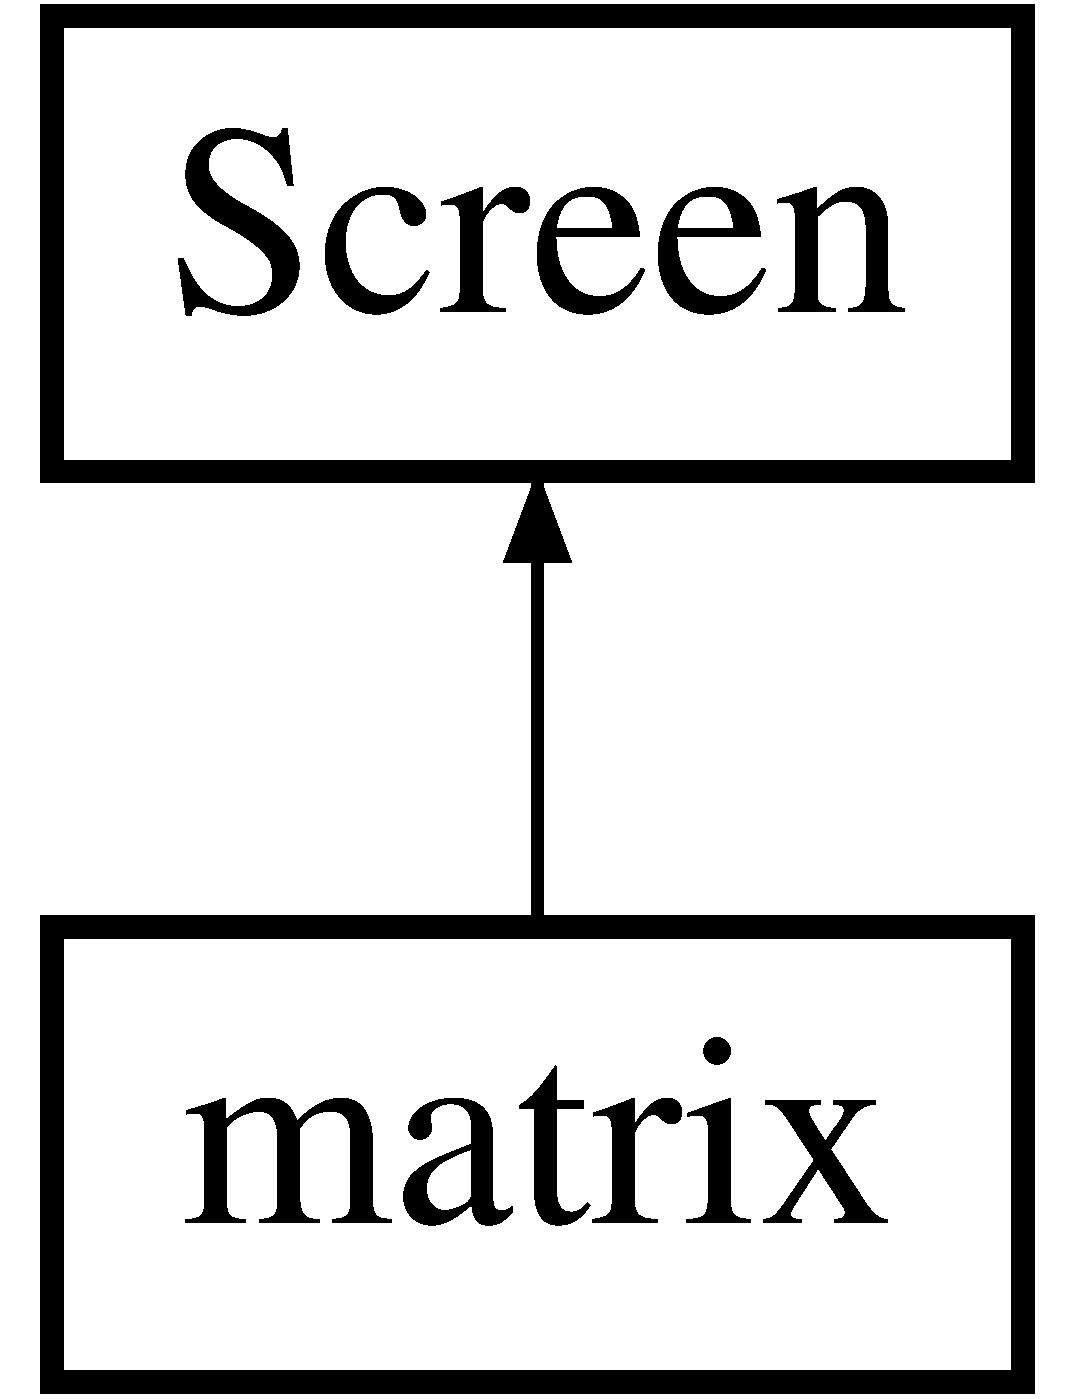
\includegraphics[height=2.000000cm]{class_screen}
\end{center}
\end{figure}
\subsection*{Public Member Functions}
\begin{DoxyCompactItemize}
\item 
\hyperlink{class_screen_a4fd315da02eebd632bdae444496c10ca}{Screen} (int w, int h)
\begin{DoxyCompactList}\small\item\em Specify the width and height of the screen. \end{DoxyCompactList}\item 
virtual void \hyperlink{class_screen_a29b3d5ac1b1f9965daa31be3acb2058e}{draw\+Pixel} (int, int, uint8\+\_\+t, uint8\+\_\+t, uint8\+\_\+t)=0
\begin{DoxyCompactList}\small\item\em Draw a given pixel with a color R G B. \end{DoxyCompactList}\item 
virtual void \hyperlink{class_screen_a01e3bb789c4169dec25e842179b7b115}{draw\+Pixel} (int, int, uint32\+\_\+t)=0
\begin{DoxyCompactList}\small\item\em Draw a pixel with a hexadecimale color. \end{DoxyCompactList}\item 
virtual void \hyperlink{class_screen_a7561ce620e5dd79717bced178e32e139}{fill\+Screen} (uint8\+\_\+t, uint8\+\_\+t, uint8\+\_\+t)
\begin{DoxyCompactList}\small\item\em Fill the entire screen with r g b colors. \end{DoxyCompactList}\item 
virtual void \hyperlink{class_screen_a6e3a21e03ec2a378c9be90b7a0a149b2}{fill\+Screen} (uint32\+\_\+t)
\begin{DoxyCompactList}\small\item\em Fill the entire screen with a hexa or decimal color. \end{DoxyCompactList}\item 
virtual void \hyperlink{class_screen_aeeb33479781ffe35c4f1c90cd66824aa}{clear} ()=0
\begin{DoxyCompactList}\small\item\em Clear the entire screen. \end{DoxyCompactList}\item 
virtual void \hyperlink{class_screen_a72c3f62745b4b863edb9e95d10057429}{start} ()
\begin{DoxyCompactList}\small\item\em Start the auto update of the screen. \end{DoxyCompactList}\item 
virtual void \hyperlink{class_screen_a38efb55f9bcb9d7181edb580ad7a77fc}{stop} ()
\begin{DoxyCompactList}\small\item\em Stop the auto update of the screen. \end{DoxyCompactList}\item 
virtual void \hyperlink{class_screen_ac609bb9d2adb5d38e077231be25c374d}{swap\+\_\+buffer} (bool copy)
\begin{DoxyCompactList}\small\item\em Swap the back buffer with front buffer. \end{DoxyCompactList}\item 
virtual void \hyperlink{class_screen_ac5346289493d80ddf429ce2369756c14}{update} ()
\item 
int \hyperlink{class_screen_ab71b25e991771611d4acab431f92b518}{get\+Width} ()
\item 
int \hyperlink{class_screen_a4edca55b221da0326dc7de0ec0f4dc91}{get\+Height} ()
\begin{DoxyCompactList}\small\item\em Return the height of the screen in pixel. \end{DoxyCompactList}\end{DoxyCompactItemize}
\subsection*{Protected Attributes}
\begin{DoxyCompactItemize}
\item 
int \hyperlink{class_screen_a49be8f8ccf7ed7a3151a761495c0ce21}{width}
\begin{DoxyCompactList}\small\item\em width and height of the screen. \end{DoxyCompactList}\item 
int \hyperlink{class_screen_a55405920693276db8fbdbf3a903b8d2f}{height}
\end{DoxyCompactItemize}


\subsection{Detailed Description}
The interface for led matrix and eventual other led screens. 

This class abstracts the interface to a led screens. You cannot define this class as an object. This class should be derieved by any class that implements a led screen. 

\subsection{Constructor \& Destructor Documentation}
\index{Screen@{Screen}!Screen@{Screen}}
\index{Screen@{Screen}!Screen@{Screen}}
\subsubsection[{\texorpdfstring{Screen(int w, int h)}{Screen(int w, int h)}}]{\setlength{\rightskip}{0pt plus 5cm}Screen\+::\+Screen (
\begin{DoxyParamCaption}
\item[{int}]{w, }
\item[{int}]{h}
\end{DoxyParamCaption}
)\hspace{0.3cm}{\ttfamily [inline]}}\hypertarget{class_screen_a4fd315da02eebd632bdae444496c10ca}{}\label{class_screen_a4fd315da02eebd632bdae444496c10ca}


Specify the width and height of the screen. 

Width and height are in pixel. 

\subsection{Member Function Documentation}
\index{Screen@{Screen}!clear@{clear}}
\index{clear@{clear}!Screen@{Screen}}
\subsubsection[{\texorpdfstring{clear()=0}{clear()=0}}]{\setlength{\rightskip}{0pt plus 5cm}virtual void Screen\+::clear (
\begin{DoxyParamCaption}
{}
\end{DoxyParamCaption}
)\hspace{0.3cm}{\ttfamily [pure virtual]}}\hypertarget{class_screen_aeeb33479781ffe35c4f1c90cd66824aa}{}\label{class_screen_aeeb33479781ffe35c4f1c90cd66824aa}


Clear the entire screen. 



Implemented in \hyperlink{classmatrix_af7e01d4f030990aba4e57af5085bd25c}{matrix}.

\index{Screen@{Screen}!draw\+Pixel@{draw\+Pixel}}
\index{draw\+Pixel@{draw\+Pixel}!Screen@{Screen}}
\subsubsection[{\texorpdfstring{draw\+Pixel(int, int, uint8\+\_\+t, uint8\+\_\+t, uint8\+\_\+t)=0}{drawPixel(int, int, uint8_t, uint8_t, uint8_t)=0}}]{\setlength{\rightskip}{0pt plus 5cm}virtual void Screen\+::draw\+Pixel (
\begin{DoxyParamCaption}
\item[{int}]{, }
\item[{int}]{, }
\item[{uint8\+\_\+t}]{, }
\item[{uint8\+\_\+t}]{, }
\item[{uint8\+\_\+t}]{}
\end{DoxyParamCaption}
)\hspace{0.3cm}{\ttfamily [pure virtual]}}\hypertarget{class_screen_a29b3d5ac1b1f9965daa31be3acb2058e}{}\label{class_screen_a29b3d5ac1b1f9965daa31be3acb2058e}


Draw a given pixel with a color R G B. 

the first int argument is the width position and the second is the height position of a pixel. rgb color is between 0 and 255. 

Implemented in \hyperlink{classmatrix_a9e12daa9f177f70cecfeae60770eb59a}{matrix}.

\index{Screen@{Screen}!draw\+Pixel@{draw\+Pixel}}
\index{draw\+Pixel@{draw\+Pixel}!Screen@{Screen}}
\subsubsection[{\texorpdfstring{draw\+Pixel(int, int, uint32\+\_\+t)=0}{drawPixel(int, int, uint32_t)=0}}]{\setlength{\rightskip}{0pt plus 5cm}virtual void Screen\+::draw\+Pixel (
\begin{DoxyParamCaption}
\item[{int}]{, }
\item[{int}]{, }
\item[{uint32\+\_\+t}]{}
\end{DoxyParamCaption}
)\hspace{0.3cm}{\ttfamily [pure virtual]}}\hypertarget{class_screen_a01e3bb789c4169dec25e842179b7b115}{}\label{class_screen_a01e3bb789c4169dec25e842179b7b115}


Draw a pixel with a hexadecimale color. 

the first int argument is the width position and the second is the height position of a pixel. color is rgb is hexa or decimale. 

Implemented in \hyperlink{classmatrix_a505fdd2958c4be8cf2ceaf19873358f9}{matrix}.

\index{Screen@{Screen}!fill\+Screen@{fill\+Screen}}
\index{fill\+Screen@{fill\+Screen}!Screen@{Screen}}
\subsubsection[{\texorpdfstring{fill\+Screen(uint8\+\_\+t, uint8\+\_\+t, uint8\+\_\+t)}{fillScreen(uint8_t, uint8_t, uint8_t)}}]{\setlength{\rightskip}{0pt plus 5cm}virtual void Screen\+::fill\+Screen (
\begin{DoxyParamCaption}
\item[{uint8\+\_\+t}]{, }
\item[{uint8\+\_\+t}]{, }
\item[{uint8\+\_\+t}]{}
\end{DoxyParamCaption}
)\hspace{0.3cm}{\ttfamily [inline]}, {\ttfamily [virtual]}}\hypertarget{class_screen_a7561ce620e5dd79717bced178e32e139}{}\label{class_screen_a7561ce620e5dd79717bced178e32e139}


Fill the entire screen with r g b colors. 



Reimplemented in \hyperlink{classmatrix_afbb1e0fe6c1ad426879c5019b39f896e}{matrix}.

\index{Screen@{Screen}!fill\+Screen@{fill\+Screen}}
\index{fill\+Screen@{fill\+Screen}!Screen@{Screen}}
\subsubsection[{\texorpdfstring{fill\+Screen(uint32\+\_\+t)}{fillScreen(uint32_t)}}]{\setlength{\rightskip}{0pt plus 5cm}virtual void Screen\+::fill\+Screen (
\begin{DoxyParamCaption}
\item[{uint32\+\_\+t}]{}
\end{DoxyParamCaption}
)\hspace{0.3cm}{\ttfamily [inline]}, {\ttfamily [virtual]}}\hypertarget{class_screen_a6e3a21e03ec2a378c9be90b7a0a149b2}{}\label{class_screen_a6e3a21e03ec2a378c9be90b7a0a149b2}


Fill the entire screen with a hexa or decimal color. 



Reimplemented in \hyperlink{classmatrix_a1a44a0f6011c61daa50391cda8d662d9}{matrix}.

\index{Screen@{Screen}!get\+Height@{get\+Height}}
\index{get\+Height@{get\+Height}!Screen@{Screen}}
\subsubsection[{\texorpdfstring{get\+Height()}{getHeight()}}]{\setlength{\rightskip}{0pt plus 5cm}int Screen\+::get\+Height (
\begin{DoxyParamCaption}
{}
\end{DoxyParamCaption}
)\hspace{0.3cm}{\ttfamily [inline]}}\hypertarget{class_screen_a4edca55b221da0326dc7de0ec0f4dc91}{}\label{class_screen_a4edca55b221da0326dc7de0ec0f4dc91}


Return the height of the screen in pixel. 

\index{Screen@{Screen}!get\+Width@{get\+Width}}
\index{get\+Width@{get\+Width}!Screen@{Screen}}
\subsubsection[{\texorpdfstring{get\+Width()}{getWidth()}}]{\setlength{\rightskip}{0pt plus 5cm}int Screen\+::get\+Width (
\begin{DoxyParamCaption}
{}
\end{DoxyParamCaption}
)\hspace{0.3cm}{\ttfamily [inline]}}\hypertarget{class_screen_ab71b25e991771611d4acab431f92b518}{}\label{class_screen_ab71b25e991771611d4acab431f92b518}
\index{Screen@{Screen}!start@{start}}
\index{start@{start}!Screen@{Screen}}
\subsubsection[{\texorpdfstring{start()}{start()}}]{\setlength{\rightskip}{0pt plus 5cm}virtual void Screen\+::start (
\begin{DoxyParamCaption}
{}
\end{DoxyParamCaption}
)\hspace{0.3cm}{\ttfamily [inline]}, {\ttfamily [virtual]}}\hypertarget{class_screen_a72c3f62745b4b863edb9e95d10057429}{}\label{class_screen_a72c3f62745b4b863edb9e95d10057429}


Start the auto update of the screen. 



Reimplemented in \hyperlink{classmatrix_a191f64280f94a2fba62ad92edf6d038a}{matrix}.

\index{Screen@{Screen}!stop@{stop}}
\index{stop@{stop}!Screen@{Screen}}
\subsubsection[{\texorpdfstring{stop()}{stop()}}]{\setlength{\rightskip}{0pt plus 5cm}virtual void Screen\+::stop (
\begin{DoxyParamCaption}
{}
\end{DoxyParamCaption}
)\hspace{0.3cm}{\ttfamily [inline]}, {\ttfamily [virtual]}}\hypertarget{class_screen_a38efb55f9bcb9d7181edb580ad7a77fc}{}\label{class_screen_a38efb55f9bcb9d7181edb580ad7a77fc}


Stop the auto update of the screen. 



Reimplemented in \hyperlink{classmatrix_a3e791088f813e071a60dca840b6b3767}{matrix}.

\index{Screen@{Screen}!swap\+\_\+buffer@{swap\+\_\+buffer}}
\index{swap\+\_\+buffer@{swap\+\_\+buffer}!Screen@{Screen}}
\subsubsection[{\texorpdfstring{swap\+\_\+buffer(bool copy)}{swap_buffer(bool copy)}}]{\setlength{\rightskip}{0pt plus 5cm}virtual void Screen\+::swap\+\_\+buffer (
\begin{DoxyParamCaption}
\item[{bool}]{copy}
\end{DoxyParamCaption}
)\hspace{0.3cm}{\ttfamily [inline]}, {\ttfamily [virtual]}}\hypertarget{class_screen_ac609bb9d2adb5d38e077231be25c374d}{}\label{class_screen_ac609bb9d2adb5d38e077231be25c374d}


Swap the back buffer with front buffer. 

You can also copy the values of new buffer to the old buffer by passing a true bool to the function. 

Reimplemented in \hyperlink{classmatrix_a371a4877409c2710021cfa3c226e63fb}{matrix}.

\index{Screen@{Screen}!update@{update}}
\index{update@{update}!Screen@{Screen}}
\subsubsection[{\texorpdfstring{update()}{update()}}]{\setlength{\rightskip}{0pt plus 5cm}virtual void Screen\+::update (
\begin{DoxyParamCaption}
\item[{void}]{}
\end{DoxyParamCaption}
)\hspace{0.3cm}{\ttfamily [inline]}, {\ttfamily [virtual]}}\hypertarget{class_screen_ac5346289493d80ddf429ce2369756c14}{}\label{class_screen_ac5346289493d80ddf429ce2369756c14}


Reimplemented in \hyperlink{classmatrix_a55827c936f54e69487cc52b83a2311c3}{matrix}.



\subsection{Member Data Documentation}
\index{Screen@{Screen}!height@{height}}
\index{height@{height}!Screen@{Screen}}
\subsubsection[{\texorpdfstring{height}{height}}]{\setlength{\rightskip}{0pt plus 5cm}int Screen\+::height\hspace{0.3cm}{\ttfamily [protected]}}\hypertarget{class_screen_a55405920693276db8fbdbf3a903b8d2f}{}\label{class_screen_a55405920693276db8fbdbf3a903b8d2f}
\index{Screen@{Screen}!width@{width}}
\index{width@{width}!Screen@{Screen}}
\subsubsection[{\texorpdfstring{width}{width}}]{\setlength{\rightskip}{0pt plus 5cm}int Screen\+::width\hspace{0.3cm}{\ttfamily [protected]}}\hypertarget{class_screen_a49be8f8ccf7ed7a3151a761495c0ce21}{}\label{class_screen_a49be8f8ccf7ed7a3151a761495c0ce21}


width and height of the screen. 



The documentation for this class was generated from the following file\+:\begin{DoxyCompactItemize}
\item 
\hyperlink{_screen_8hpp}{Screen.\+hpp}\end{DoxyCompactItemize}

\hypertarget{class_string}{}\section{String Class Reference}
\label{class_string}\index{String@{String}}


\hyperlink{class_string}{String} class implements text manipulation to be used by a \hyperlink{class_screen}{Screen} object e.\+g. matrix object.  




{\ttfamily \#include $<$String.\+hpp$>$}

Inheritance diagram for String\+:\begin{figure}[H]
\begin{center}
\leavevmode
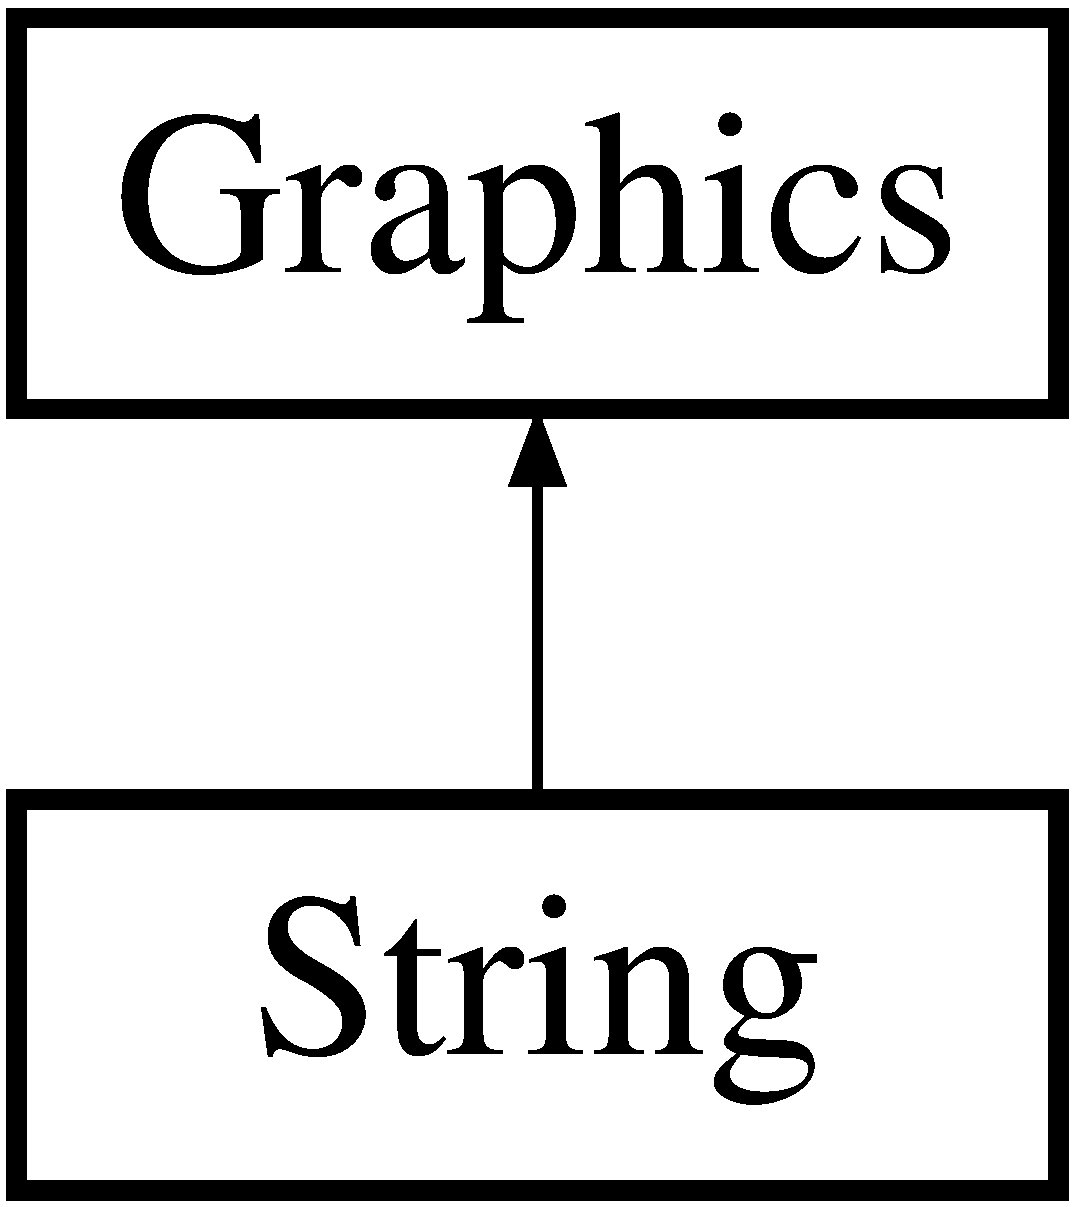
\includegraphics[height=2.000000cm]{class_string}
\end{center}
\end{figure}
\subsection*{Public Member Functions}
\begin{DoxyCompactItemize}
\item 
\hyperlink{class_string_a5fabbb03b070a2d5c6916933755b7e54}{String} (\hyperlink{class_screen}{Screen} \&\hyperlink{class_graphics_a7a73ddd0d3cf1b67fc54f303be017c3b}{w}, const uint8\+\_\+t $\ast$font, char $\ast$text, uint8\+\_\+t r, uint8\+\_\+t g, uint8\+\_\+t b, \hyperlink{classvector}{vector} \hyperlink{class_graphics_a88c2112c7a3db3ee56f4c7fe2cac6055}{location}=\hyperlink{classvector}{vector}(31, 63))
\begin{DoxyCompactList}\small\item\em \hyperlink{class_string}{String} constructor. \end{DoxyCompactList}\item 
\hyperlink{class_string_a8cb33c01999d1f29401e03980f9e6320}{String} (\hyperlink{class_screen}{Screen} \&\hyperlink{class_graphics_a7a73ddd0d3cf1b67fc54f303be017c3b}{w}, const uint8\+\_\+t $\ast$font, char $\ast$text, uint32\+\_\+t color, \hyperlink{classvector}{vector} \hyperlink{class_graphics_a88c2112c7a3db3ee56f4c7fe2cac6055}{location}=\hyperlink{classvector}{vector}(31, 63))
\begin{DoxyCompactList}\small\item\em \hyperlink{class_string}{String} constructor. \end{DoxyCompactList}\item 
void \hyperlink{class_string_a6f00d1cdc1842feb404809c717a62581}{draw} () override
\begin{DoxyCompactList}\small\item\em Print the text on the screen. \end{DoxyCompactList}\item 
void \hyperlink{class_string_a433da031c73912ed5d6e69cf64fc5f11}{scroll} (int update\+Interval=10, bool loop=false, int startX=64)
\begin{DoxyCompactList}\small\item\em Scroll text from left to right at startX. \end{DoxyCompactList}\item 
void \hyperlink{class_string_a37aa31373e430a39e216786a3a3cb929}{set\+Text} (char $\ast$t)
\begin{DoxyCompactList}\small\item\em Set the text of string. \end{DoxyCompactList}\item 
void \hyperlink{class_string_a4b35e26e6395a36833519bf351bc3567}{set\+Color} (uint32\+\_\+t c)
\begin{DoxyCompactList}\small\item\em Set the color of the string. \end{DoxyCompactList}\item 
void \hyperlink{class_string_aaece4a14fa7a17bf3f52e31e849edd87}{set\+Color} (uint8\+\_\+t rc, uint8\+\_\+t gc, uint8\+\_\+t bc)
\begin{DoxyCompactList}\small\item\em Set the color of the string. \end{DoxyCompactList}\item 
void \hyperlink{class_string_a6e7e01a0933bc9d8aeaf745c39b26020}{set\+Font} (const uint8\+\_\+t $\ast$f)
\begin{DoxyCompactList}\small\item\em Set the font of the string. \end{DoxyCompactList}\end{DoxyCompactItemize}
\subsection*{Additional Inherited Members}


\subsection{Detailed Description}
\hyperlink{class_string}{String} class implements text manipulation to be used by a \hyperlink{class_screen}{Screen} object e.\+g. matrix object. 

\hyperlink{class_string}{String} class can print a text on the screen and/or scroll it from right to left. 

\subsection{Constructor \& Destructor Documentation}
\index{String@{String}!String@{String}}
\index{String@{String}!String@{String}}
\subsubsection[{\texorpdfstring{String(\+Screen \&w, const uint8\+\_\+t $\ast$font, char $\ast$text, uint8\+\_\+t r, uint8\+\_\+t g, uint8\+\_\+t b, vector location=vector(31, 63))}{String(Screen &w, const uint8_t *font, char *text, uint8_t r, uint8_t g, uint8_t b, vector location=vector(31, 63))}}]{\setlength{\rightskip}{0pt plus 5cm}String\+::\+String (
\begin{DoxyParamCaption}
\item[{{\bf Screen} \&}]{w, }
\item[{const uint8\+\_\+t $\ast$}]{font, }
\item[{char $\ast$}]{text, }
\item[{uint8\+\_\+t}]{r, }
\item[{uint8\+\_\+t}]{g, }
\item[{uint8\+\_\+t}]{b, }
\item[{{\bf vector}}]{location = {\ttfamily {\bf vector}(31,63)}}
\end{DoxyParamCaption}
)}\hypertarget{class_string_a5fabbb03b070a2d5c6916933755b7e54}{}\label{class_string_a5fabbb03b070a2d5c6916933755b7e54}


\hyperlink{class_string}{String} constructor. 

\hyperlink{class_screen}{Screen} is the display you want to draw text on to it e.\+g. matrix. font is a font file. you need to convert the normal .ttf font with a commandline script and then include the .h file into your project. font is the name of array in that file (usually the same as the file name e.\+g. tahoma10). text is the string you want to write on the screen. You have to typecast your string first to char$\ast$. for example if you want to print \char`\"{}\+Hallo World\char`\"{} you have to pass it like this\+: (char$\ast$)\char`\"{}\+Hallo World\char`\"{}. r g b are colors of the text. they are between 0 and 255. location is the location of line you want to write text on it. The height or Y should be greater than font size to be able to see the text on screen. The characters will be printed from bottom to top. \index{String@{String}!String@{String}}
\index{String@{String}!String@{String}}
\subsubsection[{\texorpdfstring{String(\+Screen \&w, const uint8\+\_\+t $\ast$font, char $\ast$text, uint32\+\_\+t color, vector location=vector(31, 63))}{String(Screen &w, const uint8_t *font, char *text, uint32_t color, vector location=vector(31, 63))}}]{\setlength{\rightskip}{0pt plus 5cm}String\+::\+String (
\begin{DoxyParamCaption}
\item[{{\bf Screen} \&}]{w, }
\item[{const uint8\+\_\+t $\ast$}]{font, }
\item[{char $\ast$}]{text, }
\item[{uint32\+\_\+t}]{color, }
\item[{{\bf vector}}]{location = {\ttfamily {\bf vector}(31,63)}}
\end{DoxyParamCaption}
)}\hypertarget{class_string_a8cb33c01999d1f29401e03980f9e6320}{}\label{class_string_a8cb33c01999d1f29401e03980f9e6320}


\hyperlink{class_string}{String} constructor. 

\hyperlink{class_screen}{Screen} is the display you want to draw text on to it e.\+g. matrix. font is a font file. you need to convert the normal .ttf font with a commandline script and then include the .h file into your project. font is the name of array in that file (usually the same as the file name e.\+g. tahoma10). text is the string you want to write on the screen. You have to typecast your string first to char$\ast$. for example if you want to print \char`\"{}\+Hallo World\char`\"{} you have to pass it like this\+: (char$\ast$)\char`\"{}\+Hallo World\char`\"{}. color is the colors of the text. It can be max 24 bits (2$^\wedge$24-\/1). location is the location of line you want to write text on it. The height or Y should be greater than font size to be able to see the text on screen. The characters will be printed from bottom to top. 

\subsection{Member Function Documentation}
\index{String@{String}!draw@{draw}}
\index{draw@{draw}!String@{String}}
\subsubsection[{\texorpdfstring{draw() override}{draw() override}}]{\setlength{\rightskip}{0pt plus 5cm}void String\+::draw (
\begin{DoxyParamCaption}
{}
\end{DoxyParamCaption}
)\hspace{0.3cm}{\ttfamily [override]}, {\ttfamily [virtual]}}\hypertarget{class_string_a6f00d1cdc1842feb404809c717a62581}{}\label{class_string_a6f00d1cdc1842feb404809c717a62581}


Print the text on the screen. 

The characters will be printed on the screen at the specified position. Note that if double buffering is enabled you have to swap the buffers for the text to be showed on the screen. 

Implements \hyperlink{class_graphics_a144fcecfe73dd5957c081dad42e1c11d}{Graphics}.

\index{String@{String}!scroll@{scroll}}
\index{scroll@{scroll}!String@{String}}
\subsubsection[{\texorpdfstring{scroll(int update\+Interval=10, bool loop=false, int start\+X=64)}{scroll(int updateInterval=10, bool loop=false, int startX=64)}}]{\setlength{\rightskip}{0pt plus 5cm}void String\+::scroll (
\begin{DoxyParamCaption}
\item[{int}]{update\+Interval = {\ttfamily 10}, }
\item[{bool}]{loop = {\ttfamily false}, }
\item[{int}]{startX = {\ttfamily 64}}
\end{DoxyParamCaption}
)}\hypertarget{class_string_a433da031c73912ed5d6e69cf64fc5f11}{}\label{class_string_a433da031c73912ed5d6e69cf64fc5f11}


Scroll text from left to right at startX. 

This function scrolls the text from right to left at the speed of \char`\"{}update\+Interval\char`\"{}. \char`\"{}update\+Interval\char`\"{} is in milliseconds. if loop is true the scrolling of the text would be continuously. startX is width\textquotesingle{}s postion where the text start to scroll from. You do not need to swap the buffer. It\textquotesingle{}s done internally. \index{String@{String}!set\+Color@{set\+Color}}
\index{set\+Color@{set\+Color}!String@{String}}
\subsubsection[{\texorpdfstring{set\+Color(uint32\+\_\+t c)}{setColor(uint32_t c)}}]{\setlength{\rightskip}{0pt plus 5cm}void String\+::set\+Color (
\begin{DoxyParamCaption}
\item[{uint32\+\_\+t}]{c}
\end{DoxyParamCaption}
)}\hypertarget{class_string_a4b35e26e6395a36833519bf351bc3567}{}\label{class_string_a4b35e26e6395a36833519bf351bc3567}


Set the color of the string. 

This function changes the color of the text. the color can be a (hexa)decimal between 0 and 2$^\wedge$24-\/1. \index{String@{String}!set\+Color@{set\+Color}}
\index{set\+Color@{set\+Color}!String@{String}}
\subsubsection[{\texorpdfstring{set\+Color(uint8\+\_\+t rc, uint8\+\_\+t gc, uint8\+\_\+t bc)}{setColor(uint8_t rc, uint8_t gc, uint8_t bc)}}]{\setlength{\rightskip}{0pt plus 5cm}void String\+::set\+Color (
\begin{DoxyParamCaption}
\item[{uint8\+\_\+t}]{rc, }
\item[{uint8\+\_\+t}]{gc, }
\item[{uint8\+\_\+t}]{bc}
\end{DoxyParamCaption}
)}\hypertarget{class_string_aaece4a14fa7a17bf3f52e31e849edd87}{}\label{class_string_aaece4a14fa7a17bf3f52e31e849edd87}


Set the color of the string. 

This function changes the color of the text. r g and b can be between 0 and 255. \index{String@{String}!set\+Font@{set\+Font}}
\index{set\+Font@{set\+Font}!String@{String}}
\subsubsection[{\texorpdfstring{set\+Font(const uint8\+\_\+t $\ast$f)}{setFont(const uint8_t *f)}}]{\setlength{\rightskip}{0pt plus 5cm}void String\+::set\+Font (
\begin{DoxyParamCaption}
\item[{const uint8\+\_\+t $\ast$}]{f}
\end{DoxyParamCaption}
)\hspace{0.3cm}{\ttfamily [inline]}}\hypertarget{class_string_a6e7e01a0933bc9d8aeaf745c39b26020}{}\label{class_string_a6e7e01a0933bc9d8aeaf745c39b26020}


Set the font of the string. 

This function changes the font of the string. font is a font file. you need to convert the normal .ttf font with a commandline script and then include the .h file into your project. font is the name of array in that file (usually the same as the file name e.\+g. tahoma10). \index{String@{String}!set\+Text@{set\+Text}}
\index{set\+Text@{set\+Text}!String@{String}}
\subsubsection[{\texorpdfstring{set\+Text(char $\ast$t)}{setText(char *t)}}]{\setlength{\rightskip}{0pt plus 5cm}void String\+::set\+Text (
\begin{DoxyParamCaption}
\item[{char $\ast$}]{t}
\end{DoxyParamCaption}
)\hspace{0.3cm}{\ttfamily [inline]}}\hypertarget{class_string_a37aa31373e430a39e216786a3a3cb929}{}\label{class_string_a37aa31373e430a39e216786a3a3cb929}


Set the text of string. 

This function changes the text of the string. It has to be typecasted to char$\ast$. For example if you want to pass \char`\"{}\+Hallo World\char`\"{} to the function, you have to write it as\+: (char$\ast$)\char`\"{}\+Hallo World\char`\"{}. 

The documentation for this class was generated from the following files\+:\begin{DoxyCompactItemize}
\item 
\hyperlink{_string_8hpp}{String.\+hpp}\item 
\hyperlink{_string_8cpp}{String.\+cpp}\end{DoxyCompactItemize}

\hypertarget{class_timer}{}\section{Timer Class Reference}
\label{class_timer}\index{Timer@{Timer}}


\hyperlink{class_timer}{Timer} class used for wait an amount of time.  




{\ttfamily \#include $<$Timer.\+hpp$>$}

\subsection*{Public Member Functions}
\begin{DoxyCompactItemize}
\item 
\hyperlink{class_timer_a5f16e8da27d2a5a5242dead46de05d97}{Timer} ()
\begin{DoxyCompactList}\small\item\em \hyperlink{class_timer}{Timer} constructor. \end{DoxyCompactList}\item 
void \hyperlink{class_timer_ab0e4cd17c2beacc8013609ff00b8c84b}{delay\+Microseconds} (uint32\+\_\+t micro)
\begin{DoxyCompactList}\small\item\em Delay in microseconds. \end{DoxyCompactList}\item 
void \hyperlink{class_timer_a394b71189519df8fdf3f2318cf8971ef}{delay\+Milliseconds} (uint32\+\_\+t millis)
\begin{DoxyCompactList}\small\item\em Delay in milliseconds. \end{DoxyCompactList}\end{DoxyCompactItemize}


\subsection{Detailed Description}
\hyperlink{class_timer}{Timer} class used for wait an amount of time. 

\hyperlink{class_timer}{Timer} class uses \hyperlink{class_timer}{Timer} interrupt 0 channel 0. You can use only one instance at a time. 

\subsection{Constructor \& Destructor Documentation}
\index{Timer@{Timer}!Timer@{Timer}}
\index{Timer@{Timer}!Timer@{Timer}}
\subsubsection[{\texorpdfstring{Timer()}{Timer()}}]{\setlength{\rightskip}{0pt plus 5cm}Timer\+::\+Timer (
\begin{DoxyParamCaption}
{}
\end{DoxyParamCaption}
)}\hypertarget{class_timer_a5f16e8da27d2a5a5242dead46de05d97}{}\label{class_timer_a5f16e8da27d2a5a5242dead46de05d97}


\hyperlink{class_timer}{Timer} constructor. 

Configure timer interrupt 0 channel 0 to be used with a frequenty of 1 M\+HZ 

\subsection{Member Function Documentation}
\index{Timer@{Timer}!delay\+Microseconds@{delay\+Microseconds}}
\index{delay\+Microseconds@{delay\+Microseconds}!Timer@{Timer}}
\subsubsection[{\texorpdfstring{delay\+Microseconds(uint32\+\_\+t micro)}{delayMicroseconds(uint32_t micro)}}]{\setlength{\rightskip}{0pt plus 5cm}void Timer\+::delay\+Microseconds (
\begin{DoxyParamCaption}
\item[{uint32\+\_\+t}]{micro}
\end{DoxyParamCaption}
)}\hypertarget{class_timer_ab0e4cd17c2beacc8013609ff00b8c84b}{}\label{class_timer_ab0e4cd17c2beacc8013609ff00b8c84b}


Delay in microseconds. 

Delay the flow of a code by given microseconds time interval. \index{Timer@{Timer}!delay\+Milliseconds@{delay\+Milliseconds}}
\index{delay\+Milliseconds@{delay\+Milliseconds}!Timer@{Timer}}
\subsubsection[{\texorpdfstring{delay\+Milliseconds(uint32\+\_\+t millis)}{delayMilliseconds(uint32_t millis)}}]{\setlength{\rightskip}{0pt plus 5cm}void Timer\+::delay\+Milliseconds (
\begin{DoxyParamCaption}
\item[{uint32\+\_\+t}]{millis}
\end{DoxyParamCaption}
)}\hypertarget{class_timer_a394b71189519df8fdf3f2318cf8971ef}{}\label{class_timer_a394b71189519df8fdf3f2318cf8971ef}


Delay in milliseconds. 

Delay the flow of a code by given milliseconds time interval. 

The documentation for this class was generated from the following files\+:\begin{DoxyCompactItemize}
\item 
\hyperlink{_timer_8hpp}{Timer.\+hpp}\item 
\hyperlink{_timer_8cpp}{Timer.\+cpp}\end{DoxyCompactItemize}

\hypertarget{classvector}{}\section{vector Class Reference}
\label{classvector}\index{vector@{vector}}


Implementation of vector class to store x and y.  




{\ttfamily \#include $<$vector.\+hpp$>$}

\subsection*{Public Member Functions}
\begin{DoxyCompactItemize}
\item 
\hyperlink{classvector_a7fa147d3199381b9d8b32753bd1a6968}{vector} (int \hyperlink{classvector_a0403eb3aea23a3009e276fba1d317046}{x}, int \hyperlink{classvector_aad6de640298eae97ca0a094db5aff477}{y})
\item 
\hyperlink{classvector_a829904aef4f1a78fc3c52ef7c857f8f4}{vector} (const \hyperlink{classvector}{vector} \&rhs)
\item 
\hyperlink{classvector}{vector} \& \hyperlink{classvector_acf4c6a4d343c92e211f80de7712a3cac}{operator+=} (const \hyperlink{classvector}{vector} \&rhs)
\item 
\hyperlink{classvector}{vector} \hyperlink{classvector_a2ab7f62262c6f0c6ade3bd1879e6001e}{operator+} (const \hyperlink{classvector}{vector} \&rhs) const 
\item 
\hyperlink{classvector}{vector} \& \hyperlink{classvector_a9f6cf8d24ca60a5bec617c364172d89f}{operator-\/=} (const \hyperlink{classvector}{vector} \&rhs)
\item 
\hyperlink{classvector}{vector} \hyperlink{classvector_ad9596a53b6aef33bbddfa7b9b4b17f09}{operator-\/} (const \hyperlink{classvector}{vector} \&rhs) const 
\item 
\hyperlink{classvector}{vector} \& \hyperlink{classvector_a6adc3766a4afa03340fa2a94d6d81a00}{operator$\ast$=} (int n)
\item 
\hyperlink{classvector}{vector} \hyperlink{classvector_ac69d5833c619427c28a8fb120d30b5c8}{operator$\ast$} (int n) const 
\end{DoxyCompactItemize}
\subsection*{Public Attributes}
\begin{DoxyCompactItemize}
\item 
int \hyperlink{classvector_a0403eb3aea23a3009e276fba1d317046}{x}
\item 
int \hyperlink{classvector_aad6de640298eae97ca0a094db5aff477}{y}
\end{DoxyCompactItemize}


\subsection{Detailed Description}
Implementation of vector class to store x and y. 

This class used by several classes in this library to store x and y or width and height. 

\subsection{Constructor \& Destructor Documentation}
\index{vector@{vector}!vector@{vector}}
\index{vector@{vector}!vector@{vector}}
\subsubsection[{\texorpdfstring{vector(int x, int y)}{vector(int x, int y)}}]{\setlength{\rightskip}{0pt plus 5cm}vector\+::vector (
\begin{DoxyParamCaption}
\item[{int}]{x, }
\item[{int}]{y}
\end{DoxyParamCaption}
)\hspace{0.3cm}{\ttfamily [inline]}}\hypertarget{classvector_a7fa147d3199381b9d8b32753bd1a6968}{}\label{classvector_a7fa147d3199381b9d8b32753bd1a6968}
\index{vector@{vector}!vector@{vector}}
\index{vector@{vector}!vector@{vector}}
\subsubsection[{\texorpdfstring{vector(const vector \&rhs)}{vector(const vector &rhs)}}]{\setlength{\rightskip}{0pt plus 5cm}vector\+::vector (
\begin{DoxyParamCaption}
\item[{const {\bf vector} \&}]{rhs}
\end{DoxyParamCaption}
)\hspace{0.3cm}{\ttfamily [inline]}}\hypertarget{classvector_a829904aef4f1a78fc3c52ef7c857f8f4}{}\label{classvector_a829904aef4f1a78fc3c52ef7c857f8f4}


\subsection{Member Function Documentation}
\index{vector@{vector}!operator$\ast$@{operator$\ast$}}
\index{operator$\ast$@{operator$\ast$}!vector@{vector}}
\subsubsection[{\texorpdfstring{operator$\ast$(int n) const }{operator*(int n) const }}]{\setlength{\rightskip}{0pt plus 5cm}{\bf vector} vector\+::operator$\ast$ (
\begin{DoxyParamCaption}
\item[{int}]{n}
\end{DoxyParamCaption}
) const\hspace{0.3cm}{\ttfamily [inline]}}\hypertarget{classvector_ac69d5833c619427c28a8fb120d30b5c8}{}\label{classvector_ac69d5833c619427c28a8fb120d30b5c8}
\index{vector@{vector}!operator$\ast$=@{operator$\ast$=}}
\index{operator$\ast$=@{operator$\ast$=}!vector@{vector}}
\subsubsection[{\texorpdfstring{operator$\ast$=(int n)}{operator*=(int n)}}]{\setlength{\rightskip}{0pt plus 5cm}{\bf vector}\& vector\+::operator$\ast$= (
\begin{DoxyParamCaption}
\item[{int}]{n}
\end{DoxyParamCaption}
)\hspace{0.3cm}{\ttfamily [inline]}}\hypertarget{classvector_a6adc3766a4afa03340fa2a94d6d81a00}{}\label{classvector_a6adc3766a4afa03340fa2a94d6d81a00}
\index{vector@{vector}!operator+@{operator+}}
\index{operator+@{operator+}!vector@{vector}}
\subsubsection[{\texorpdfstring{operator+(const vector \&rhs) const }{operator+(const vector &rhs) const }}]{\setlength{\rightskip}{0pt plus 5cm}{\bf vector} vector\+::operator+ (
\begin{DoxyParamCaption}
\item[{const {\bf vector} \&}]{rhs}
\end{DoxyParamCaption}
) const\hspace{0.3cm}{\ttfamily [inline]}}\hypertarget{classvector_a2ab7f62262c6f0c6ade3bd1879e6001e}{}\label{classvector_a2ab7f62262c6f0c6ade3bd1879e6001e}
\index{vector@{vector}!operator+=@{operator+=}}
\index{operator+=@{operator+=}!vector@{vector}}
\subsubsection[{\texorpdfstring{operator+=(const vector \&rhs)}{operator+=(const vector &rhs)}}]{\setlength{\rightskip}{0pt plus 5cm}{\bf vector}\& vector\+::operator+= (
\begin{DoxyParamCaption}
\item[{const {\bf vector} \&}]{rhs}
\end{DoxyParamCaption}
)\hspace{0.3cm}{\ttfamily [inline]}}\hypertarget{classvector_acf4c6a4d343c92e211f80de7712a3cac}{}\label{classvector_acf4c6a4d343c92e211f80de7712a3cac}
\index{vector@{vector}!operator-\/@{operator-\/}}
\index{operator-\/@{operator-\/}!vector@{vector}}
\subsubsection[{\texorpdfstring{operator-\/(const vector \&rhs) const }{operator-(const vector &rhs) const }}]{\setlength{\rightskip}{0pt plus 5cm}{\bf vector} vector\+::operator-\/ (
\begin{DoxyParamCaption}
\item[{const {\bf vector} \&}]{rhs}
\end{DoxyParamCaption}
) const\hspace{0.3cm}{\ttfamily [inline]}}\hypertarget{classvector_ad9596a53b6aef33bbddfa7b9b4b17f09}{}\label{classvector_ad9596a53b6aef33bbddfa7b9b4b17f09}
\index{vector@{vector}!operator-\/=@{operator-\/=}}
\index{operator-\/=@{operator-\/=}!vector@{vector}}
\subsubsection[{\texorpdfstring{operator-\/=(const vector \&rhs)}{operator-=(const vector &rhs)}}]{\setlength{\rightskip}{0pt plus 5cm}{\bf vector}\& vector\+::operator-\/= (
\begin{DoxyParamCaption}
\item[{const {\bf vector} \&}]{rhs}
\end{DoxyParamCaption}
)\hspace{0.3cm}{\ttfamily [inline]}}\hypertarget{classvector_a9f6cf8d24ca60a5bec617c364172d89f}{}\label{classvector_a9f6cf8d24ca60a5bec617c364172d89f}


\subsection{Member Data Documentation}
\index{vector@{vector}!x@{x}}
\index{x@{x}!vector@{vector}}
\subsubsection[{\texorpdfstring{x}{x}}]{\setlength{\rightskip}{0pt plus 5cm}int vector\+::x}\hypertarget{classvector_a0403eb3aea23a3009e276fba1d317046}{}\label{classvector_a0403eb3aea23a3009e276fba1d317046}
\index{vector@{vector}!y@{y}}
\index{y@{y}!vector@{vector}}
\subsubsection[{\texorpdfstring{y}{y}}]{\setlength{\rightskip}{0pt plus 5cm}int vector\+::y}\hypertarget{classvector_aad6de640298eae97ca0a094db5aff477}{}\label{classvector_aad6de640298eae97ca0a094db5aff477}


The documentation for this class was generated from the following file\+:\begin{DoxyCompactItemize}
\item 
\hyperlink{vector_8hpp}{vector.\+hpp}\end{DoxyCompactItemize}

\chapter{File Documentation}
\hypertarget{_animated_image_8cpp}{}\section{Animated\+Image.\+cpp File Reference}
\label{_animated_image_8cpp}\index{Animated\+Image.\+cpp@{Animated\+Image.\+cpp}}
{\ttfamily \#include \char`\"{}Animated\+Image.\+hpp\char`\"{}}\\*

\hypertarget{_animated_image_8hpp}{}\section{Animated\+Image.\+hpp File Reference}
\label{_animated_image_8hpp}\index{Animated\+Image.\+hpp@{Animated\+Image.\+hpp}}
{\ttfamily \#include \char`\"{}Graphics.\+hpp\char`\"{}}\\*
{\ttfamily \#include \char`\"{}Timer.\+hpp\char`\"{}}\\*
\subsection*{Classes}
\begin{DoxyCompactItemize}
\item 
class \hyperlink{class_animated_image}{Animated\+Image}
\begin{DoxyCompactList}\small\item\em Animate\+Image implementation for raw gif files. \end{DoxyCompactList}\end{DoxyCompactItemize}

\hypertarget{doxygen_8hpp}{}\section{doxygen.\+hpp File Reference}
\label{doxygen_8hpp}\index{doxygen.\+hpp@{doxygen.\+hpp}}

\hypertarget{gamma_8h}{}\section{gamma.\+h File Reference}
\label{gamma_8h}\index{gamma.\+h@{gamma.\+h}}
{\ttfamily \#include $<$stdint.\+h$>$}\\*
\subsection*{Variables}
\begin{DoxyCompactItemize}
\item 
const uint8\+\_\+t \hyperlink{gamma_8h_a4a355960fc13a7e0520b3141f8820dba}{gamma} \mbox{[}256\mbox{]}
\end{DoxyCompactItemize}


\subsection{Variable Documentation}
\index{gamma.\+h@{gamma.\+h}!gamma@{gamma}}
\index{gamma@{gamma}!gamma.\+h@{gamma.\+h}}
\subsubsection[{\texorpdfstring{gamma}{gamma}}]{\setlength{\rightskip}{0pt plus 5cm}const uint8\+\_\+t gamma\mbox{[}256\mbox{]}}\hypertarget{gamma_8h_a4a355960fc13a7e0520b3141f8820dba}{}\label{gamma_8h_a4a355960fc13a7e0520b3141f8820dba}

\hypertarget{gamma__generator_8c}{}\section{gamma\+\_\+generator.\+c File Reference}
\label{gamma__generator_8c}\index{gamma\+\_\+generator.\+c@{gamma\+\_\+generator.\+c}}
{\ttfamily \#include $<$stdio.\+h$>$}\\*
{\ttfamily \#include $<$math.\+h$>$}\\*
\subsection*{Macros}
\begin{DoxyCompactItemize}
\item 
\#define \hyperlink{gamma__generator_8c_a8659b9de3e544ff142b153b076f30fd5}{G\+A\+M\+MA}~2.\+5
\end{DoxyCompactItemize}
\subsection*{Functions}
\begin{DoxyCompactItemize}
\item 
int \hyperlink{gamma__generator_8c_a0ddf1224851353fc92bfbff6f499fa97}{main} (int argc, char $\ast$argv\mbox{[}$\,$\mbox{]})
\end{DoxyCompactItemize}
\subsection*{Variables}
\begin{DoxyCompactItemize}
\item 
int \hyperlink{gamma__generator_8c_a04c7177f8eeaf2c1a2166e9637ee5497}{planes} = 8
\end{DoxyCompactItemize}


\subsection{Macro Definition Documentation}
\index{gamma\+\_\+generator.\+c@{gamma\+\_\+generator.\+c}!G\+A\+M\+MA@{G\+A\+M\+MA}}
\index{G\+A\+M\+MA@{G\+A\+M\+MA}!gamma\+\_\+generator.\+c@{gamma\+\_\+generator.\+c}}
\subsubsection[{\texorpdfstring{G\+A\+M\+MA}{GAMMA}}]{\setlength{\rightskip}{0pt plus 5cm}\#define G\+A\+M\+MA~2.\+5}\hypertarget{gamma__generator_8c_a8659b9de3e544ff142b153b076f30fd5}{}\label{gamma__generator_8c_a8659b9de3e544ff142b153b076f30fd5}


\subsection{Function Documentation}
\index{gamma\+\_\+generator.\+c@{gamma\+\_\+generator.\+c}!main@{main}}
\index{main@{main}!gamma\+\_\+generator.\+c@{gamma\+\_\+generator.\+c}}
\subsubsection[{\texorpdfstring{main(int argc, char $\ast$argv[])}{main(int argc, char *argv[])}}]{\setlength{\rightskip}{0pt plus 5cm}int main (
\begin{DoxyParamCaption}
\item[{int}]{argc, }
\item[{char $\ast$}]{argv\mbox{[}$\,$\mbox{]}}
\end{DoxyParamCaption}
)}\hypertarget{gamma__generator_8c_a0ddf1224851353fc92bfbff6f499fa97}{}\label{gamma__generator_8c_a0ddf1224851353fc92bfbff6f499fa97}


\subsection{Variable Documentation}
\index{gamma\+\_\+generator.\+c@{gamma\+\_\+generator.\+c}!planes@{planes}}
\index{planes@{planes}!gamma\+\_\+generator.\+c@{gamma\+\_\+generator.\+c}}
\subsubsection[{\texorpdfstring{planes}{planes}}]{\setlength{\rightskip}{0pt plus 5cm}int planes = 8}\hypertarget{gamma__generator_8c_a04c7177f8eeaf2c1a2166e9637ee5497}{}\label{gamma__generator_8c_a04c7177f8eeaf2c1a2166e9637ee5497}

\hypertarget{_graphics_8hpp}{}\section{Graphics.\+hpp File Reference}
\label{_graphics_8hpp}\index{Graphics.\+hpp@{Graphics.\+hpp}}
{\ttfamily \#include \char`\"{}vector.\+hpp\char`\"{}}\\*
{\ttfamily \#include \char`\"{}Screen.\+hpp\char`\"{}}\\*
\subsection*{Classes}
\begin{DoxyCompactItemize}
\item 
class \hyperlink{class_graphics}{Graphics}
\begin{DoxyCompactList}\small\item\em The interface for other graphics objects. \end{DoxyCompactList}\end{DoxyCompactItemize}

\hypertarget{_image_8cpp}{}\section{Image.\+cpp File Reference}
\label{_image_8cpp}\index{Image.\+cpp@{Image.\+cpp}}
{\ttfamily \#include \char`\"{}Image.\+hpp\char`\"{}}\\*

\hypertarget{_image_8hpp}{}\section{Image.\+hpp File Reference}
\label{_image_8hpp}\index{Image.\+hpp@{Image.\+hpp}}
{\ttfamily \#include \char`\"{}Graphics.\+hpp\char`\"{}}\\*
\subsection*{Classes}
\begin{DoxyCompactItemize}
\item 
class \hyperlink{class_image}{Image}
\begin{DoxyCompactList}\small\item\em Implementation for raw image files. \end{DoxyCompactList}\end{DoxyCompactItemize}

\hypertarget{init_8c}{}\section{init.\+c File Reference}
\label{init_8c}\index{init.\+c@{init.\+c}}
{\ttfamily \#include \char`\"{}sam3xa.\+h\char`\"{}}\\*
\subsection*{Macros}
\begin{DoxyCompactItemize}
\item 
\#define \hyperlink{init_8c_a0a22f8ffd78d8577790c0ccf7471e06d}{S\+Y\+S\+\_\+\+B\+O\+A\+R\+D\+\_\+\+O\+S\+C\+O\+U\+NT}~(C\+K\+G\+R\+\_\+\+M\+O\+R\+\_\+\+M\+O\+S\+C\+X\+T\+ST(0x8))
\item 
\#define \hyperlink{init_8c_aed7d52452ed405bce522ac60f0a9526c}{S\+Y\+S\+\_\+\+B\+O\+A\+R\+D\+\_\+\+P\+L\+L\+AR}~(C\+K\+G\+R\+\_\+\+P\+L\+L\+A\+R\+\_\+\+O\+NE $\vert$ C\+K\+G\+R\+\_\+\+P\+L\+L\+A\+R\+\_\+\+M\+U\+LA(0xd\+U\+L) $\vert$ C\+K\+G\+R\+\_\+\+P\+L\+L\+A\+R\+\_\+\+P\+L\+L\+A\+C\+O\+U\+N\+T(0x3f\+U\+L) $\vert$ C\+K\+G\+R\+\_\+\+P\+L\+L\+A\+R\+\_\+\+D\+I\+V\+A(0x1\+U\+L))
\item 
\#define \hyperlink{init_8c_a5723ea67fd327e388188538ae2db2f66}{S\+Y\+S\+\_\+\+B\+O\+A\+R\+D\+\_\+\+M\+C\+KR}~(P\+M\+C\+\_\+\+M\+C\+K\+R\+\_\+\+P\+R\+E\+S\+\_\+\+C\+L\+K\+\_\+2 $\vert$ P\+M\+C\+\_\+\+M\+C\+K\+R\+\_\+\+C\+S\+S\+\_\+\+P\+L\+L\+A\+\_\+\+C\+LK)
\end{DoxyCompactItemize}
\subsection*{Functions}
\begin{DoxyCompactItemize}
\item 
void \hyperlink{init_8c_adc86b84eeabe5d8dc8445cec2314d925}{system\+Init} ()
\end{DoxyCompactItemize}


\subsection{Macro Definition Documentation}
\index{init.\+c@{init.\+c}!S\+Y\+S\+\_\+\+B\+O\+A\+R\+D\+\_\+\+M\+C\+KR@{S\+Y\+S\+\_\+\+B\+O\+A\+R\+D\+\_\+\+M\+C\+KR}}
\index{S\+Y\+S\+\_\+\+B\+O\+A\+R\+D\+\_\+\+M\+C\+KR@{S\+Y\+S\+\_\+\+B\+O\+A\+R\+D\+\_\+\+M\+C\+KR}!init.\+c@{init.\+c}}
\subsubsection[{\texorpdfstring{S\+Y\+S\+\_\+\+B\+O\+A\+R\+D\+\_\+\+M\+C\+KR}{SYS_BOARD_MCKR}}]{\setlength{\rightskip}{0pt plus 5cm}\#define S\+Y\+S\+\_\+\+B\+O\+A\+R\+D\+\_\+\+M\+C\+KR~(P\+M\+C\+\_\+\+M\+C\+K\+R\+\_\+\+P\+R\+E\+S\+\_\+\+C\+L\+K\+\_\+2 $\vert$ P\+M\+C\+\_\+\+M\+C\+K\+R\+\_\+\+C\+S\+S\+\_\+\+P\+L\+L\+A\+\_\+\+C\+LK)}\hypertarget{init_8c_a5723ea67fd327e388188538ae2db2f66}{}\label{init_8c_a5723ea67fd327e388188538ae2db2f66}
\index{init.\+c@{init.\+c}!S\+Y\+S\+\_\+\+B\+O\+A\+R\+D\+\_\+\+O\+S\+C\+O\+U\+NT@{S\+Y\+S\+\_\+\+B\+O\+A\+R\+D\+\_\+\+O\+S\+C\+O\+U\+NT}}
\index{S\+Y\+S\+\_\+\+B\+O\+A\+R\+D\+\_\+\+O\+S\+C\+O\+U\+NT@{S\+Y\+S\+\_\+\+B\+O\+A\+R\+D\+\_\+\+O\+S\+C\+O\+U\+NT}!init.\+c@{init.\+c}}
\subsubsection[{\texorpdfstring{S\+Y\+S\+\_\+\+B\+O\+A\+R\+D\+\_\+\+O\+S\+C\+O\+U\+NT}{SYS_BOARD_OSCOUNT}}]{\setlength{\rightskip}{0pt plus 5cm}\#define S\+Y\+S\+\_\+\+B\+O\+A\+R\+D\+\_\+\+O\+S\+C\+O\+U\+NT~(C\+K\+G\+R\+\_\+\+M\+O\+R\+\_\+\+M\+O\+S\+C\+X\+T\+ST(0x8))}\hypertarget{init_8c_a0a22f8ffd78d8577790c0ccf7471e06d}{}\label{init_8c_a0a22f8ffd78d8577790c0ccf7471e06d}
\index{init.\+c@{init.\+c}!S\+Y\+S\+\_\+\+B\+O\+A\+R\+D\+\_\+\+P\+L\+L\+AR@{S\+Y\+S\+\_\+\+B\+O\+A\+R\+D\+\_\+\+P\+L\+L\+AR}}
\index{S\+Y\+S\+\_\+\+B\+O\+A\+R\+D\+\_\+\+P\+L\+L\+AR@{S\+Y\+S\+\_\+\+B\+O\+A\+R\+D\+\_\+\+P\+L\+L\+AR}!init.\+c@{init.\+c}}
\subsubsection[{\texorpdfstring{S\+Y\+S\+\_\+\+B\+O\+A\+R\+D\+\_\+\+P\+L\+L\+AR}{SYS_BOARD_PLLAR}}]{\setlength{\rightskip}{0pt plus 5cm}\#define S\+Y\+S\+\_\+\+B\+O\+A\+R\+D\+\_\+\+P\+L\+L\+AR~(C\+K\+G\+R\+\_\+\+P\+L\+L\+A\+R\+\_\+\+O\+NE $\vert$ C\+K\+G\+R\+\_\+\+P\+L\+L\+A\+R\+\_\+\+M\+U\+LA(0xd\+U\+L) $\vert$ C\+K\+G\+R\+\_\+\+P\+L\+L\+A\+R\+\_\+\+P\+L\+L\+A\+C\+O\+U\+N\+T(0x3f\+U\+L) $\vert$ C\+K\+G\+R\+\_\+\+P\+L\+L\+A\+R\+\_\+\+D\+I\+V\+A(0x1\+U\+L))}\hypertarget{init_8c_aed7d52452ed405bce522ac60f0a9526c}{}\label{init_8c_aed7d52452ed405bce522ac60f0a9526c}


\subsection{Function Documentation}
\index{init.\+c@{init.\+c}!system\+Init@{system\+Init}}
\index{system\+Init@{system\+Init}!init.\+c@{init.\+c}}
\subsubsection[{\texorpdfstring{system\+Init()}{systemInit()}}]{\setlength{\rightskip}{0pt plus 5cm}void system\+Init (
\begin{DoxyParamCaption}
{}
\end{DoxyParamCaption}
)}\hypertarget{init_8c_adc86b84eeabe5d8dc8445cec2314d925}{}\label{init_8c_adc86b84eeabe5d8dc8445cec2314d925}

\hypertarget{matrix_8cpp}{}\section{matrix.\+cpp File Reference}
\label{matrix_8cpp}\index{matrix.\+cpp@{matrix.\+cpp}}
{\ttfamily \#include \char`\"{}matrix.\+hpp\char`\"{}}\\*
{\ttfamily \#include $<$cstring$>$}\\*
\subsection*{Functions}
\begin{DoxyCompactItemize}
\item 
void \hyperlink{matrix_8cpp_ae69893861c9ce728a475a17e26296582}{T\+C3\+\_\+\+Handler} (void)
\end{DoxyCompactItemize}


\subsection{Function Documentation}
\index{matrix.\+cpp@{matrix.\+cpp}!T\+C3\+\_\+\+Handler@{T\+C3\+\_\+\+Handler}}
\index{T\+C3\+\_\+\+Handler@{T\+C3\+\_\+\+Handler}!matrix.\+cpp@{matrix.\+cpp}}
\subsubsection[{\texorpdfstring{T\+C3\+\_\+\+Handler(void)}{TC3_Handler(void)}}]{\setlength{\rightskip}{0pt plus 5cm}void T\+C3\+\_\+\+Handler (
\begin{DoxyParamCaption}
\item[{void}]{}
\end{DoxyParamCaption}
)}\hypertarget{matrix_8cpp_ae69893861c9ce728a475a17e26296582}{}\label{matrix_8cpp_ae69893861c9ce728a475a17e26296582}

\hypertarget{matrix_8hpp}{}\section{matrix.\+hpp File Reference}
\label{matrix_8hpp}\index{matrix.\+hpp@{matrix.\+hpp}}
{\ttfamily \#include \char`\"{}hwlib.\+hpp\char`\"{}}\\*
{\ttfamily \#include \char`\"{}Screen.\+hpp\char`\"{}}\\*
{\ttfamily \#include \char`\"{}gamma.\+h\char`\"{}}\\*
{\ttfamily \#include \char`\"{}Image.\+hpp\char`\"{}}\\*
{\ttfamily \#include \char`\"{}String.\+hpp\char`\"{}}\\*
{\ttfamily \#include \char`\"{}Timer.\+hpp\char`\"{}}\\*
{\ttfamily \#include \char`\"{}Animated\+Image.\+hpp\char`\"{}}\\*
{\ttfamily \#include \char`\"{}vector.\+hpp\char`\"{}}\\*
\subsection*{Classes}
\begin{DoxyCompactItemize}
\item 
class \hyperlink{classmatrix}{matrix}
\begin{DoxyCompactList}\small\item\em Led matrix implementation for the abstract class \hyperlink{class_screen}{Screen}. \end{DoxyCompactList}\end{DoxyCompactItemize}
\subsection*{Macros}
\begin{DoxyCompactItemize}
\item 
\#define \hyperlink{matrix_8hpp_a8ffc48994309205a718c137fa68c9267}{C\+B\+IT}~8
\item 
\#define \hyperlink{matrix_8hpp_ac6f18a9e1d00b4637522b1b469a92021}{R\+OW}~16
\item 
\#define \hyperlink{matrix_8hpp_ab00f2b8e8bad4307cf0775a5520cf663}{C\+OL}~512
\end{DoxyCompactItemize}


\subsection{Macro Definition Documentation}
\index{matrix.\+hpp@{matrix.\+hpp}!C\+B\+IT@{C\+B\+IT}}
\index{C\+B\+IT@{C\+B\+IT}!matrix.\+hpp@{matrix.\+hpp}}
\subsubsection[{\texorpdfstring{C\+B\+IT}{CBIT}}]{\setlength{\rightskip}{0pt plus 5cm}\#define C\+B\+IT~8}\hypertarget{matrix_8hpp_a8ffc48994309205a718c137fa68c9267}{}\label{matrix_8hpp_a8ffc48994309205a718c137fa68c9267}
\index{matrix.\+hpp@{matrix.\+hpp}!C\+OL@{C\+OL}}
\index{C\+OL@{C\+OL}!matrix.\+hpp@{matrix.\+hpp}}
\subsubsection[{\texorpdfstring{C\+OL}{COL}}]{\setlength{\rightskip}{0pt plus 5cm}\#define C\+OL~512}\hypertarget{matrix_8hpp_ab00f2b8e8bad4307cf0775a5520cf663}{}\label{matrix_8hpp_ab00f2b8e8bad4307cf0775a5520cf663}
\index{matrix.\+hpp@{matrix.\+hpp}!R\+OW@{R\+OW}}
\index{R\+OW@{R\+OW}!matrix.\+hpp@{matrix.\+hpp}}
\subsubsection[{\texorpdfstring{R\+OW}{ROW}}]{\setlength{\rightskip}{0pt plus 5cm}\#define R\+OW~16}\hypertarget{matrix_8hpp_ac6f18a9e1d00b4637522b1b469a92021}{}\label{matrix_8hpp_ac6f18a9e1d00b4637522b1b469a92021}

\hypertarget{_screen_8hpp}{}\section{Screen.\+hpp File Reference}
\label{_screen_8hpp}\index{Screen.\+hpp@{Screen.\+hpp}}
{\ttfamily \#include $<$stdint.\+h$>$}\\*
\subsection*{Classes}
\begin{DoxyCompactItemize}
\item 
class \hyperlink{class_screen}{Screen}
\begin{DoxyCompactList}\small\item\em The interface for led matrix and eventual other led screens. \end{DoxyCompactList}\end{DoxyCompactItemize}

\hypertarget{startup__sam3xa_8c}{}\section{startup\+\_\+sam3xa.\+c File Reference}
\label{startup__sam3xa_8c}\index{startup\+\_\+sam3xa.\+c@{startup\+\_\+sam3xa.\+c}}
{\ttfamily \#include \char`\"{}sam3xa.\+h\char`\"{}}\\*
\subsection*{Functions}
\begin{DoxyCompactItemize}
\item 
void \hyperlink{startup__sam3xa_8c_a5f388c8556f7cb6a84b5692db6b6ad80}{\+\_\+\+\_\+libc\+\_\+init\+\_\+array} (void)
\item 
void \hyperlink{startup__sam3xa_8c_a4ed9b32000d3b15c46ffd748f32ed44d}{Dummy\+\_\+\+Handler} (void)
\begin{DoxyCompactList}\small\item\em Default interrupt handler for unused I\+R\+Qs. \end{DoxyCompactList}\item 
void \hyperlink{startup__sam3xa_8c_aaa1400c15ada51a2aeaa13813e9f0c0d}{N\+M\+I\+\_\+\+Handler} (void Hard\+Fault\+\_\+\+Handler void)
\item 
void \hyperlink{startup__sam3xa_8c_ae7ee340978f5c25f52f0cad1457c6616}{Reset\+\_\+\+Handler} (void)
\begin{DoxyCompactList}\small\item\em This is the code that gets called on processor reset. To initialize the device, and call the \hyperlink{gamma__generator_8c_a0ddf1224851353fc92bfbff6f499fa97}{main()} routine. \end{DoxyCompactList}\end{DoxyCompactItemize}
\subsection*{Variables}
\begin{DoxyCompactItemize}
\item 
uint32\+\_\+t \hyperlink{startup__sam3xa_8c_a28a1e6a5ea108ce1447beccdd47c83c1}{\+\_\+\+\_\+stack\+\_\+end}
\end{DoxyCompactItemize}


\subsection{Function Documentation}
\index{startup\+\_\+sam3xa.\+c@{startup\+\_\+sam3xa.\+c}!\+\_\+\+\_\+libc\+\_\+init\+\_\+array@{\+\_\+\+\_\+libc\+\_\+init\+\_\+array}}
\index{\+\_\+\+\_\+libc\+\_\+init\+\_\+array@{\+\_\+\+\_\+libc\+\_\+init\+\_\+array}!startup\+\_\+sam3xa.\+c@{startup\+\_\+sam3xa.\+c}}
\subsubsection[{\texorpdfstring{\+\_\+\+\_\+libc\+\_\+init\+\_\+array(void)}{__libc_init_array(void)}}]{\setlength{\rightskip}{0pt plus 5cm}void \+\_\+\+\_\+libc\+\_\+init\+\_\+array (
\begin{DoxyParamCaption}
\item[{void}]{}
\end{DoxyParamCaption}
)}\hypertarget{startup__sam3xa_8c_a5f388c8556f7cb6a84b5692db6b6ad80}{}\label{startup__sam3xa_8c_a5f388c8556f7cb6a84b5692db6b6ad80}
\index{startup\+\_\+sam3xa.\+c@{startup\+\_\+sam3xa.\+c}!Dummy\+\_\+\+Handler@{Dummy\+\_\+\+Handler}}
\index{Dummy\+\_\+\+Handler@{Dummy\+\_\+\+Handler}!startup\+\_\+sam3xa.\+c@{startup\+\_\+sam3xa.\+c}}
\subsubsection[{\texorpdfstring{Dummy\+\_\+\+Handler(void)}{Dummy_Handler(void)}}]{\setlength{\rightskip}{0pt plus 5cm}void Dummy\+\_\+\+Handler (
\begin{DoxyParamCaption}
\item[{void}]{}
\end{DoxyParamCaption}
)}\hypertarget{startup__sam3xa_8c_a4ed9b32000d3b15c46ffd748f32ed44d}{}\label{startup__sam3xa_8c_a4ed9b32000d3b15c46ffd748f32ed44d}


Default interrupt handler for unused I\+R\+Qs. 

\index{startup\+\_\+sam3xa.\+c@{startup\+\_\+sam3xa.\+c}!N\+M\+I\+\_\+\+Handler@{N\+M\+I\+\_\+\+Handler}}
\index{N\+M\+I\+\_\+\+Handler@{N\+M\+I\+\_\+\+Handler}!startup\+\_\+sam3xa.\+c@{startup\+\_\+sam3xa.\+c}}
\subsubsection[{\texorpdfstring{N\+M\+I\+\_\+\+Handler(void Hard\+Fault\+\_\+\+Handler void)}{NMI_Handler(void HardFault_Handler void)}}]{\setlength{\rightskip}{0pt plus 5cm}void N\+M\+I\+\_\+\+Handler (
\begin{DoxyParamCaption}
\item[{void Hard\+Fault\+\_\+\+Handler}]{void}
\end{DoxyParamCaption}
)}\hypertarget{startup__sam3xa_8c_aaa1400c15ada51a2aeaa13813e9f0c0d}{}\label{startup__sam3xa_8c_aaa1400c15ada51a2aeaa13813e9f0c0d}
\index{startup\+\_\+sam3xa.\+c@{startup\+\_\+sam3xa.\+c}!Reset\+\_\+\+Handler@{Reset\+\_\+\+Handler}}
\index{Reset\+\_\+\+Handler@{Reset\+\_\+\+Handler}!startup\+\_\+sam3xa.\+c@{startup\+\_\+sam3xa.\+c}}
\subsubsection[{\texorpdfstring{Reset\+\_\+\+Handler(void)}{Reset_Handler(void)}}]{\setlength{\rightskip}{0pt plus 5cm}void Reset\+\_\+\+Handler (
\begin{DoxyParamCaption}
\item[{void}]{}
\end{DoxyParamCaption}
)}\hypertarget{startup__sam3xa_8c_ae7ee340978f5c25f52f0cad1457c6616}{}\label{startup__sam3xa_8c_ae7ee340978f5c25f52f0cad1457c6616}


This is the code that gets called on processor reset. To initialize the device, and call the \hyperlink{gamma__generator_8c_a0ddf1224851353fc92bfbff6f499fa97}{main()} routine. 



\subsection{Variable Documentation}
\index{startup\+\_\+sam3xa.\+c@{startup\+\_\+sam3xa.\+c}!\+\_\+\+\_\+stack\+\_\+end@{\+\_\+\+\_\+stack\+\_\+end}}
\index{\+\_\+\+\_\+stack\+\_\+end@{\+\_\+\+\_\+stack\+\_\+end}!startup\+\_\+sam3xa.\+c@{startup\+\_\+sam3xa.\+c}}
\subsubsection[{\texorpdfstring{\+\_\+\+\_\+stack\+\_\+end}{__stack_end}}]{\setlength{\rightskip}{0pt plus 5cm}uint32\+\_\+t \+\_\+\+\_\+stack\+\_\+end}\hypertarget{startup__sam3xa_8c_a28a1e6a5ea108ce1447beccdd47c83c1}{}\label{startup__sam3xa_8c_a28a1e6a5ea108ce1447beccdd47c83c1}

\hypertarget{_string_8cpp}{}\section{String.\+cpp File Reference}
\label{_string_8cpp}\index{String.\+cpp@{String.\+cpp}}
{\ttfamily \#include \char`\"{}String.\+hpp\char`\"{}}\\*
{\ttfamily \#include \char`\"{}Timer.\+hpp\char`\"{}}\\*

\hypertarget{_string_8hpp}{}\section{String.\+hpp File Reference}
\label{_string_8hpp}\index{String.\+hpp@{String.\+hpp}}
{\ttfamily \#include \char`\"{}Graphics.\+hpp\char`\"{}}\\*
\subsection*{Classes}
\begin{DoxyCompactItemize}
\item 
class \hyperlink{class_string}{String}
\begin{DoxyCompactList}\small\item\em \hyperlink{class_string}{String} class implements text manipulation to be used by a \hyperlink{class_screen}{Screen} object e.\+g. matrix object. \end{DoxyCompactList}\end{DoxyCompactItemize}

\hypertarget{_timer_8cpp}{}\section{Timer.\+cpp File Reference}
\label{_timer_8cpp}\index{Timer.\+cpp@{Timer.\+cpp}}
{\ttfamily \#include \char`\"{}Timer.\+hpp\char`\"{}}\\*
\subsection*{Functions}
\begin{DoxyCompactItemize}
\item 
void \hyperlink{_timer_8cpp_a2eca52a9a80dbd2067f9dbbba597f63f}{T\+C0\+\_\+\+Handler} (void)
\end{DoxyCompactItemize}


\subsection{Function Documentation}
\index{Timer.\+cpp@{Timer.\+cpp}!T\+C0\+\_\+\+Handler@{T\+C0\+\_\+\+Handler}}
\index{T\+C0\+\_\+\+Handler@{T\+C0\+\_\+\+Handler}!Timer.\+cpp@{Timer.\+cpp}}
\subsubsection[{\texorpdfstring{T\+C0\+\_\+\+Handler(void)}{TC0_Handler(void)}}]{\setlength{\rightskip}{0pt plus 5cm}void T\+C0\+\_\+\+Handler (
\begin{DoxyParamCaption}
\item[{void}]{}
\end{DoxyParamCaption}
)}\hypertarget{_timer_8cpp_a2eca52a9a80dbd2067f9dbbba597f63f}{}\label{_timer_8cpp_a2eca52a9a80dbd2067f9dbbba597f63f}

\hypertarget{_timer_8hpp}{}\section{Timer.\+hpp File Reference}
\label{_timer_8hpp}\index{Timer.\+hpp@{Timer.\+hpp}}
{\ttfamily \#include \char`\"{}hwlib.\+hpp\char`\"{}}\\*
\subsection*{Classes}
\begin{DoxyCompactItemize}
\item 
class \hyperlink{class_timer}{Timer}
\begin{DoxyCompactList}\small\item\em \hyperlink{class_timer}{Timer} class used for wait an amount of time. \end{DoxyCompactList}\end{DoxyCompactItemize}

\hypertarget{vector_8hpp}{}\section{vector.\+hpp File Reference}
\label{vector_8hpp}\index{vector.\+hpp@{vector.\+hpp}}
\subsection*{Classes}
\begin{DoxyCompactItemize}
\item 
class \hyperlink{classvector}{vector}
\begin{DoxyCompactList}\small\item\em Implementation of vector class to store x and y. \end{DoxyCompactList}\end{DoxyCompactItemize}

%--- End generated contents ---

% Index
\backmatter
\newpage
\phantomsection
\clearemptydoublepage
\addcontentsline{toc}{chapter}{Index}
\printindex

\end{document}
